\chapter{Hadron recoil calibration}\label{sec:HadrCalib}
\etmiss affects significantly the W boson measurement, so it is important to have a solid understanding  of possible of sources differences in the hadron recoil reconstruction in data and Monte Carlo. 

\begin{figure}

\begin{minipage}[h]{0.49\linewidth}
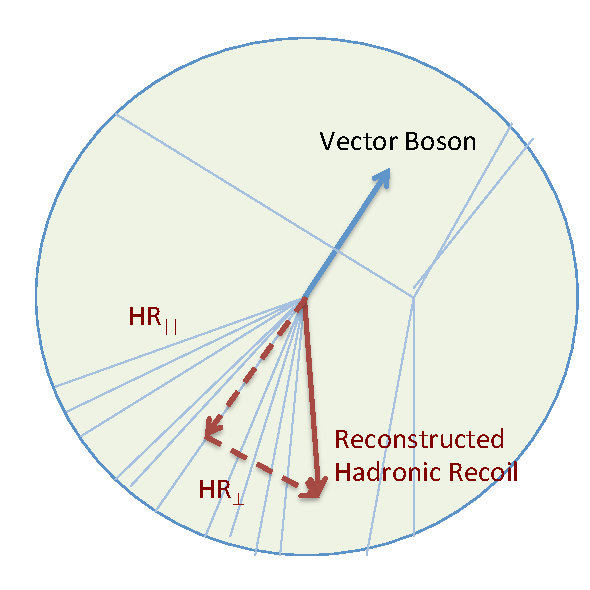
\includegraphics[width=1\textwidth]{HadronRecoil/RecoHRParPerp.pdf}
\end{minipage}

\end{figure}

The hadron recoil algorithm performance can be studied in MC through the projection of $\vec{HR}$ on the direction of the transverse momentum of the vector boson, as shown in Fig. \ref{ris:HadrRecoilTruthPt}. This projection can be divided into perpendicular \uperp and parallel \upar component as follows:
\begin{equation}
\upar=\vec{v_{xy}}\cdot\vec{HR}
\end{equation}
\begin{equation}
\uperp=v_x\cdot HR_y - v_y \cdot HR_x,
\end{equation}
where $\vec{v_{xy}}$ is a unitary vector along the transverse component of a vector boson momentum and $v_x$ and $v_y$ are its projections on x and y axis respectively. In the case of the true kinematics $\upar=p_T^{bos}$ and $\uperp = 0$. However the calorimeter resolution is causing relatively wide distributions for these projections. The parallel component \upar is sensitive to a possible bias in the hadron recoil, while the perpendicular \uperp can be used for determination of the resolution discrepancies. The mean and the width of these distributions can depend on different variables, such as a mean number of interactions in event, hadronic activity, boson $P_{T}^{bos}$ etc. 

 
It is convinient to use Z boson decays for a hadron recoil calibration, since its transverse momentum can be determined not only by a hadron recoil, but also from its decay products.  Zpt resolution coming from lepton reconstruction is 3-4 times better, than from a hadron recoil. This is allowing to treat leptonically reconstructed $P_T^{Z}$ as a truth $P_T$ of the boson and compare directly \uperp and \upar in data and MC. Small size of the Z sample in 2.76TeV data will lead to a high statistics error for this distributions. Also, calibration constants can be also derived from W boson decays through the indirect measurments. This corrections can be biased by a possible truth boson $P_T$ mismodelling. 
 
 First step in a hadron recoil calibration procedure ames to correct differences in a pile-up modelling in the event. Additional interaction can have a significant effect on a \etmiss and \sumet distributions.   It is usually accounted scaling average number of interaction per bunch crossing to match a data. However, \atlas simulation is suited for an high pile-up runs, so this quantity is modelled discretly in case of 2.76 TeV analysis (Fig. \ref{HadrRecoil:mu}), what makes the corrections to match data impossible. 

The combined Z and W boson determination procedure have been used. This section describes a procedure of calibrating bias and resolution mismodelling in a hadron recoil, that was apapted for 2.76 TeV data. 

\section{Hadron recoil resolution correction}


\begin{figure}[!tbp]
\centering
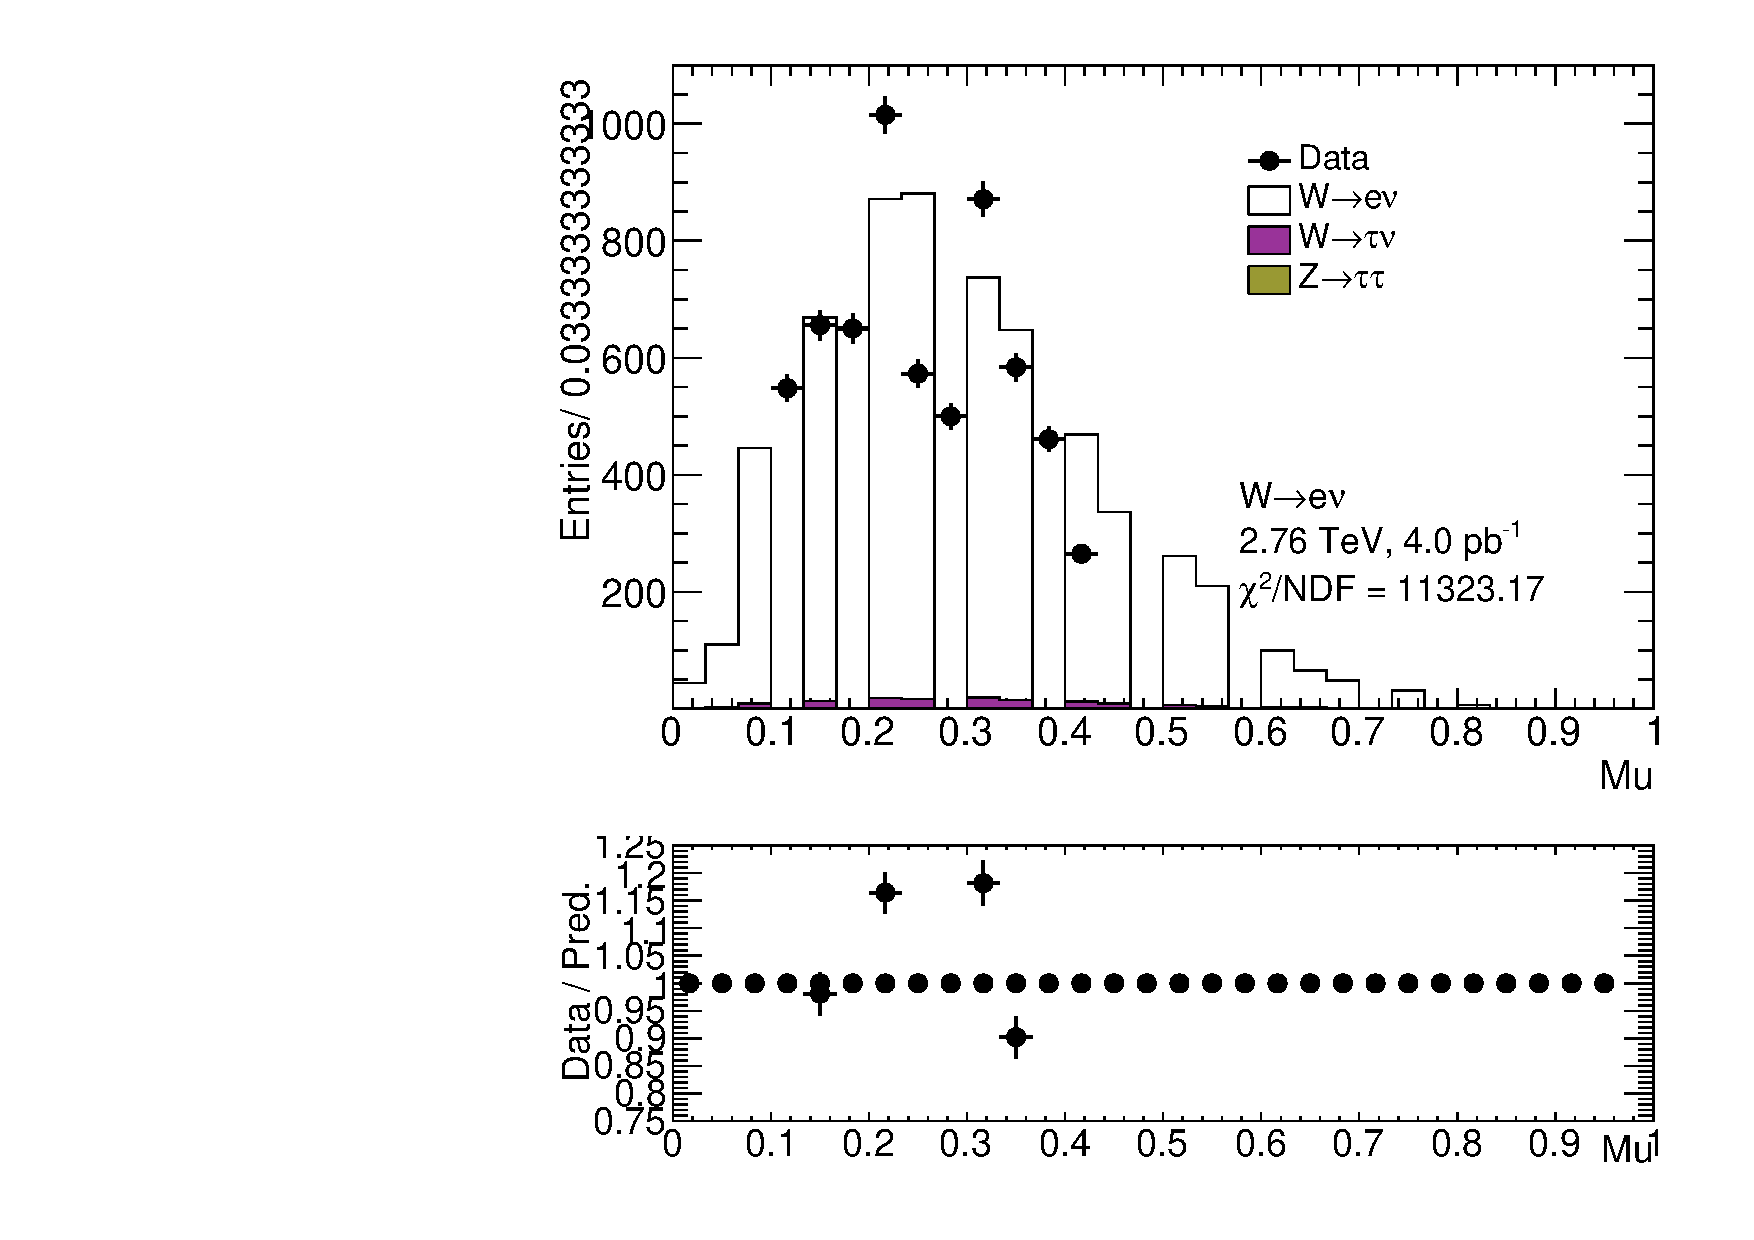
\includegraphics[width=0.5\textwidth]{HadronRecoil/W_Event_Mu.pdf}
\caption{Pileup}
\label{HadrRecoil:mu}
\end{figure} 

Event activity plays an important role in a \etmiss reconstruction. Since \sumet and hadron recoil resolution values are correlated, the possible mismodelling of event activity can lead to a differences between data and monte carlo \etmiss resolution (Fig. \ref{ris:sumetCor}). There are two possible ways of resolution correction in a 2.76 TeV data. It could be corrected by reweigting \sumet distribution to match a data. Remaining differences can be corrected on a second step. On another hand it is also possible to neglect second order effects on \etmiss from \sumet distribution and directly correct difference between data and MC. 

\begin{figure}[!tbp]
\begin{center}

\begin{minipage}[h]{0.7\linewidth}
\center{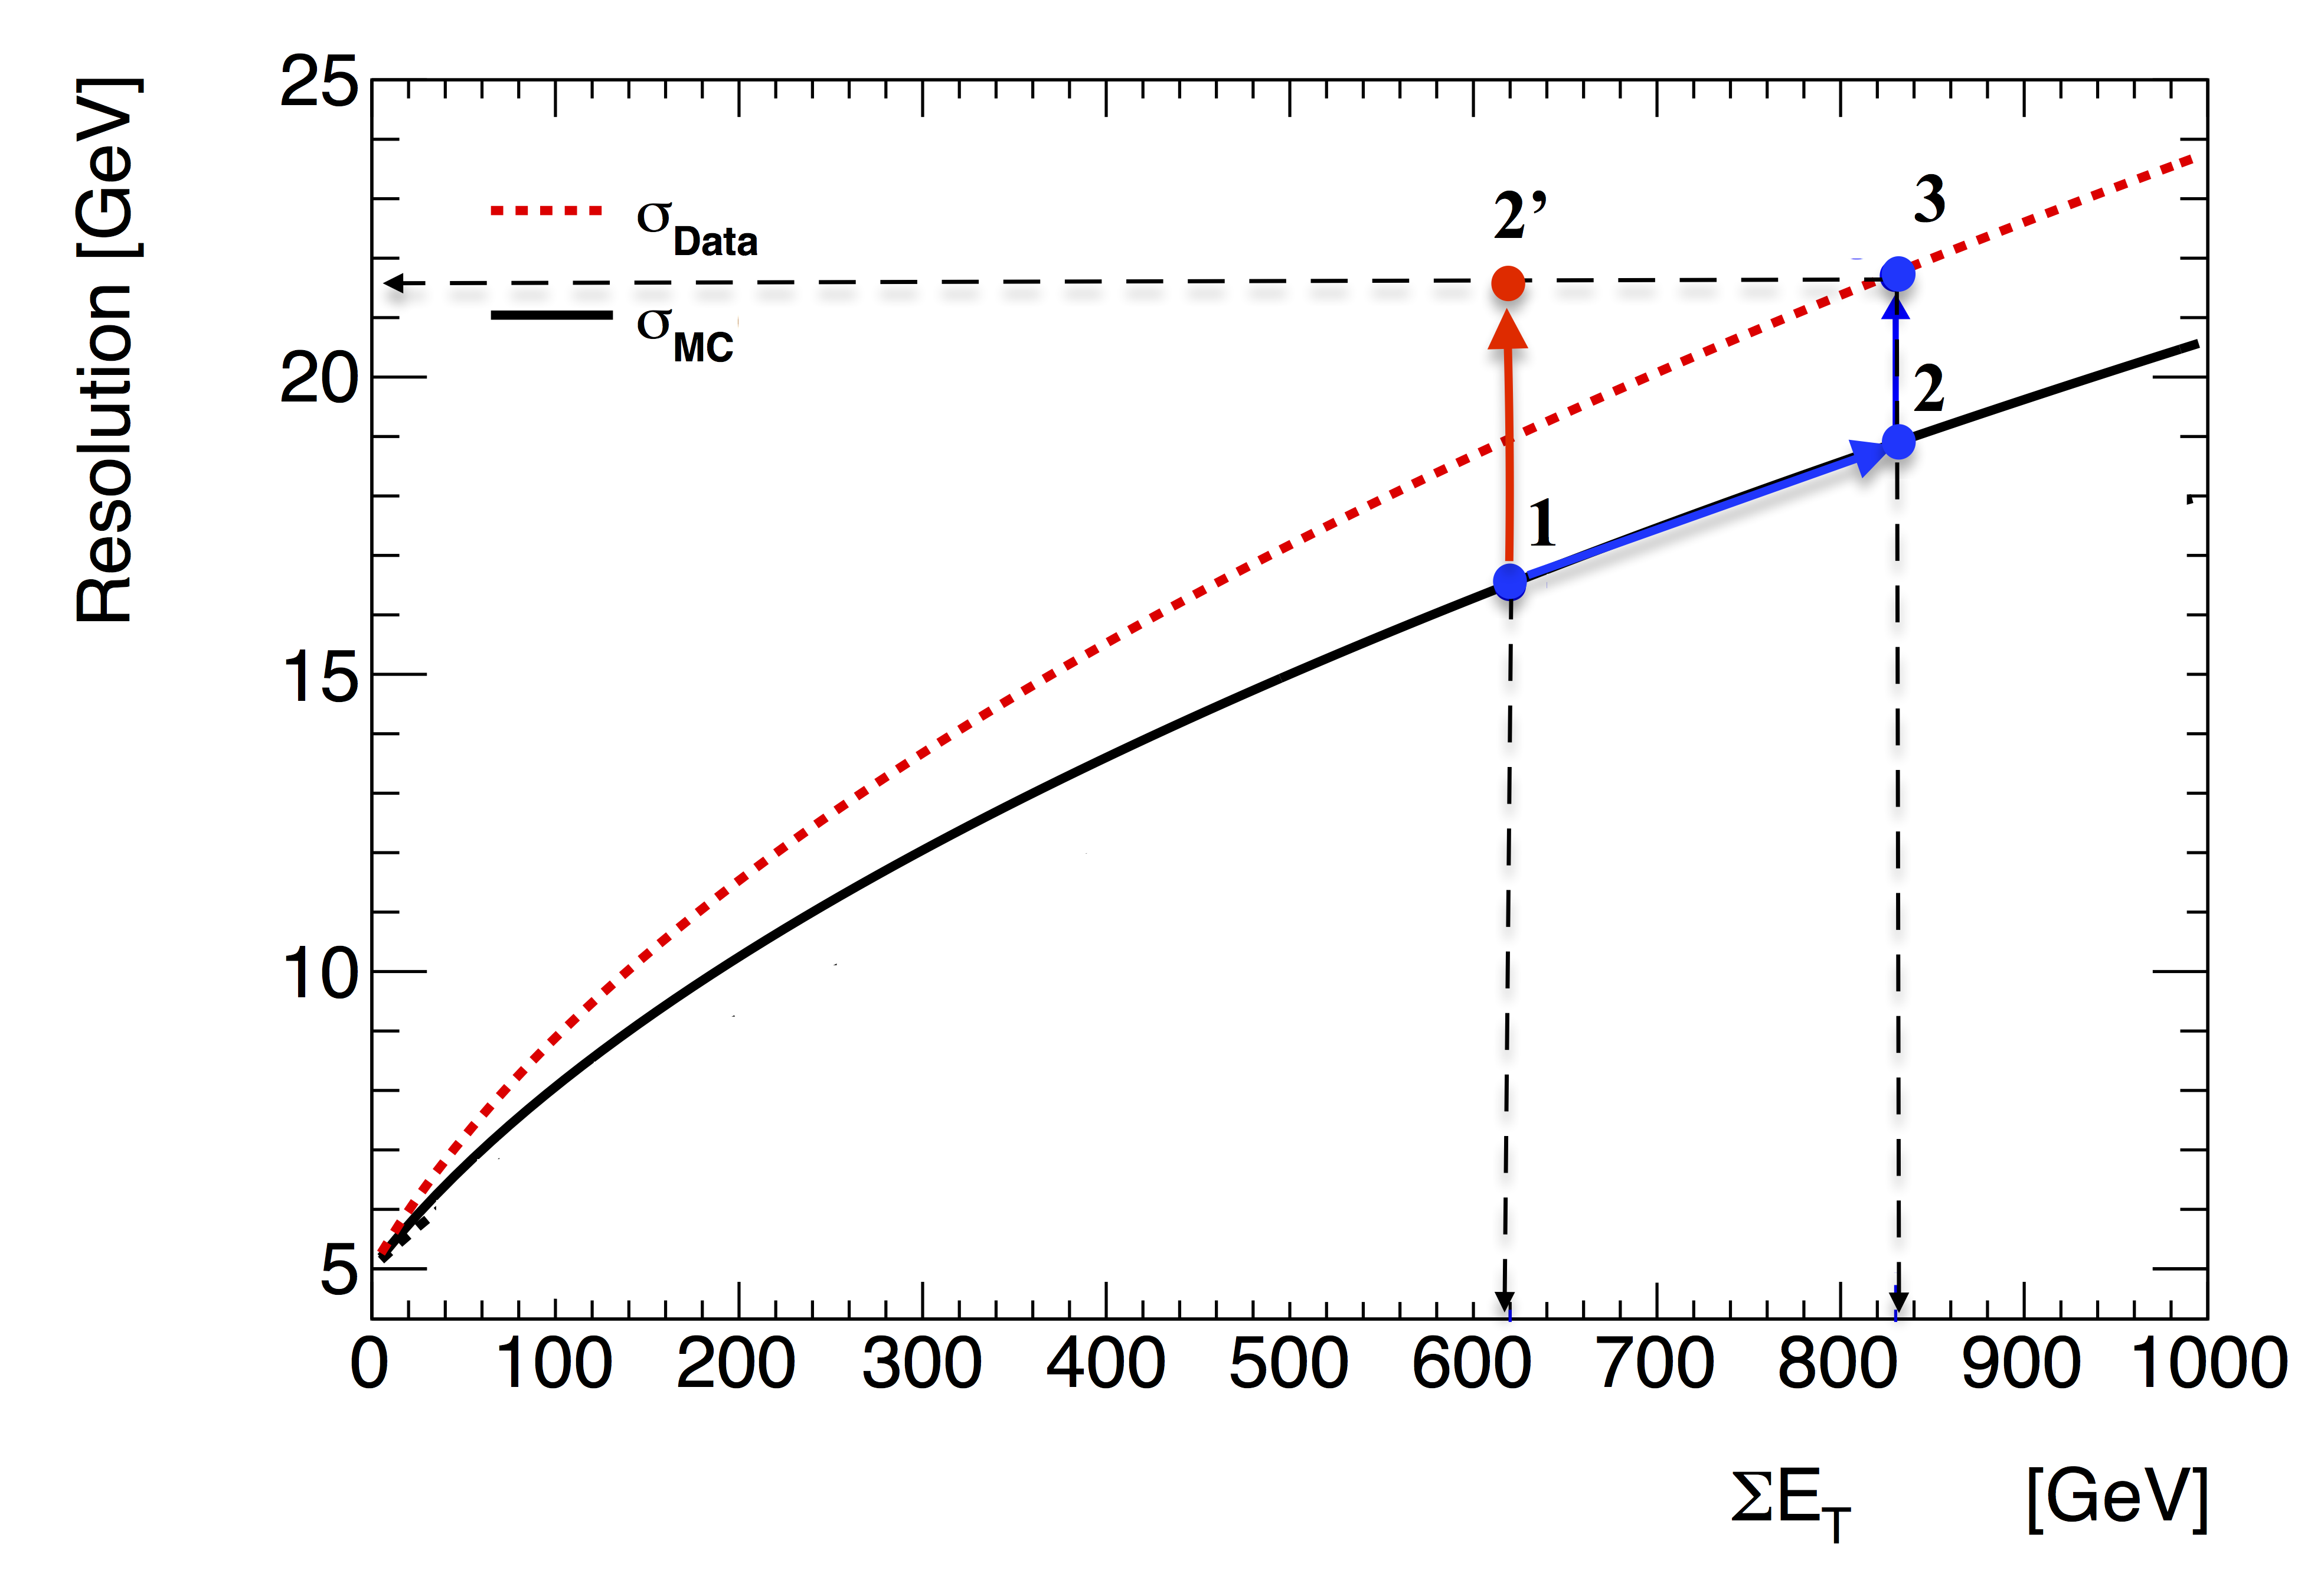
\includegraphics[width=1.\linewidth]{HadronRecoil/sumet.png}}
\end{minipage}

\end{center}
\caption{Schematic view of the correction procedure: this figure illustrates the resolution of \uperp as a function of \sumet. The dotted curve represents data resolution ($\sigma_{data}$), solid black is a nominal MC ($\sigma_{MC}$). Blue line from point 1 to point 2 corresponds to a \sumet correction. Red line from point 1 to point 2' corresponds to a direct correction of resolution mismodelling }

\label{ris:sumetCor}
\end{figure}


\begin{figure}[!tbp]
\begin{minipage}[h]{0.49\linewidth}
\center{\includegraphics[width=1.\linewidth]{HadronRecoil/UncorrSumet/W_EtMiss_CorRecoilSumet.pdf} \\ a)}
\end{minipage}
\hfill
\begin{minipage}[h]{0.49\linewidth}
\center{\includegraphics[width=1.\linewidth]{HadronRecoil/UncorrSumet/Wmu_EtMiss_CorRecoilSumet.pdf} \\ b)}
\end{minipage}
\caption{Distribution of \sumet from a) \wenu and b) \wmunu events before correction}
\label{HadrRecoil:UncorrSumet}
\vfill
\begin{minipage}[h]{0.49\linewidth}
\center{\includegraphics[width=1.\linewidth]{HadronRecoil/CorrSumet/W_EtMiss_CorRecoilSumet.pdf} \\ a)}
\end{minipage}
\hfill
\begin{minipage}[h]{0.49\linewidth}
\center{\includegraphics[width=1.\linewidth]{HadronRecoil/CorrSumet/Wmu_EtMiss_CorRecoilSumet.pdf} \\ b)}
\end{minipage}
\caption{Distribution of \sumet from a) \wenu and b) \wmunu events after correction}
\label{HadrRecoil:CorrSumet}
\end{figure}

\subsection{Sumet distribution correction}

Distribution of \sumet  events are shown on a Fig. \ref{HadrRecoil:UncorrSumet}. There is a clear sign of shift in this distribution in a both channels. Unfortunatelly, size of the Z sample is not sufficient for correcting this discrepancies. 
The determination of sumet reweighting constants uses W boson decays. Since \sumet and \ptw are correlated correction factors are derived inside $p_T^{W, rec}$  as follows:
\begin{equation}
SF^{channel}=\frac{\sum E_T^{data, \, selection} }{\sum E_T^{MC,\, no\, cuts} },
\end{equation}
where $\sum E_T^{data,\, selection} $ and $\sum E_T^{MC,\, no\, cuts}$ is a \sumet distribution inside $p_T^{W, rec}$ bin without any cuts.  Because of the small data statistics combination of  \wenu and \wmunu processes is used. Oppositely, in MC $\sum E_T^{MC,\, no\, cuts} $ is taken without any cuts. Scale factors are determined separately for each signal process for a W boson decays. Example of correction factors for a different $p_T^{W, rec}$ bins are shown on a Fig.\ref{ris:SumEtCorPtW} Ratio inside each bin can be parameterised by a polynomial degree 2 inside each $p_T^{W, rec}$ bin.  Total SF obtained by this procedure are shown on a Fig. \ref{SFWplusenu}. The distribution of \sumet after correction is shown on a Fig. \ref{HadrRecoil:CorrSumet}. Reconstructed boson pt spectrum is leaving almost untouched, while this procedure still intoduses some shift in a truth boson pt spectrum(Fig. \ref{HadrRecoil:PtSpectrum} ). Effect on the resoultion of \uperp is shown on a Fig. \ref{something}.
\begin{figure}[!tbp]
\begin{minipage}[h]{0.49\linewidth}
\center{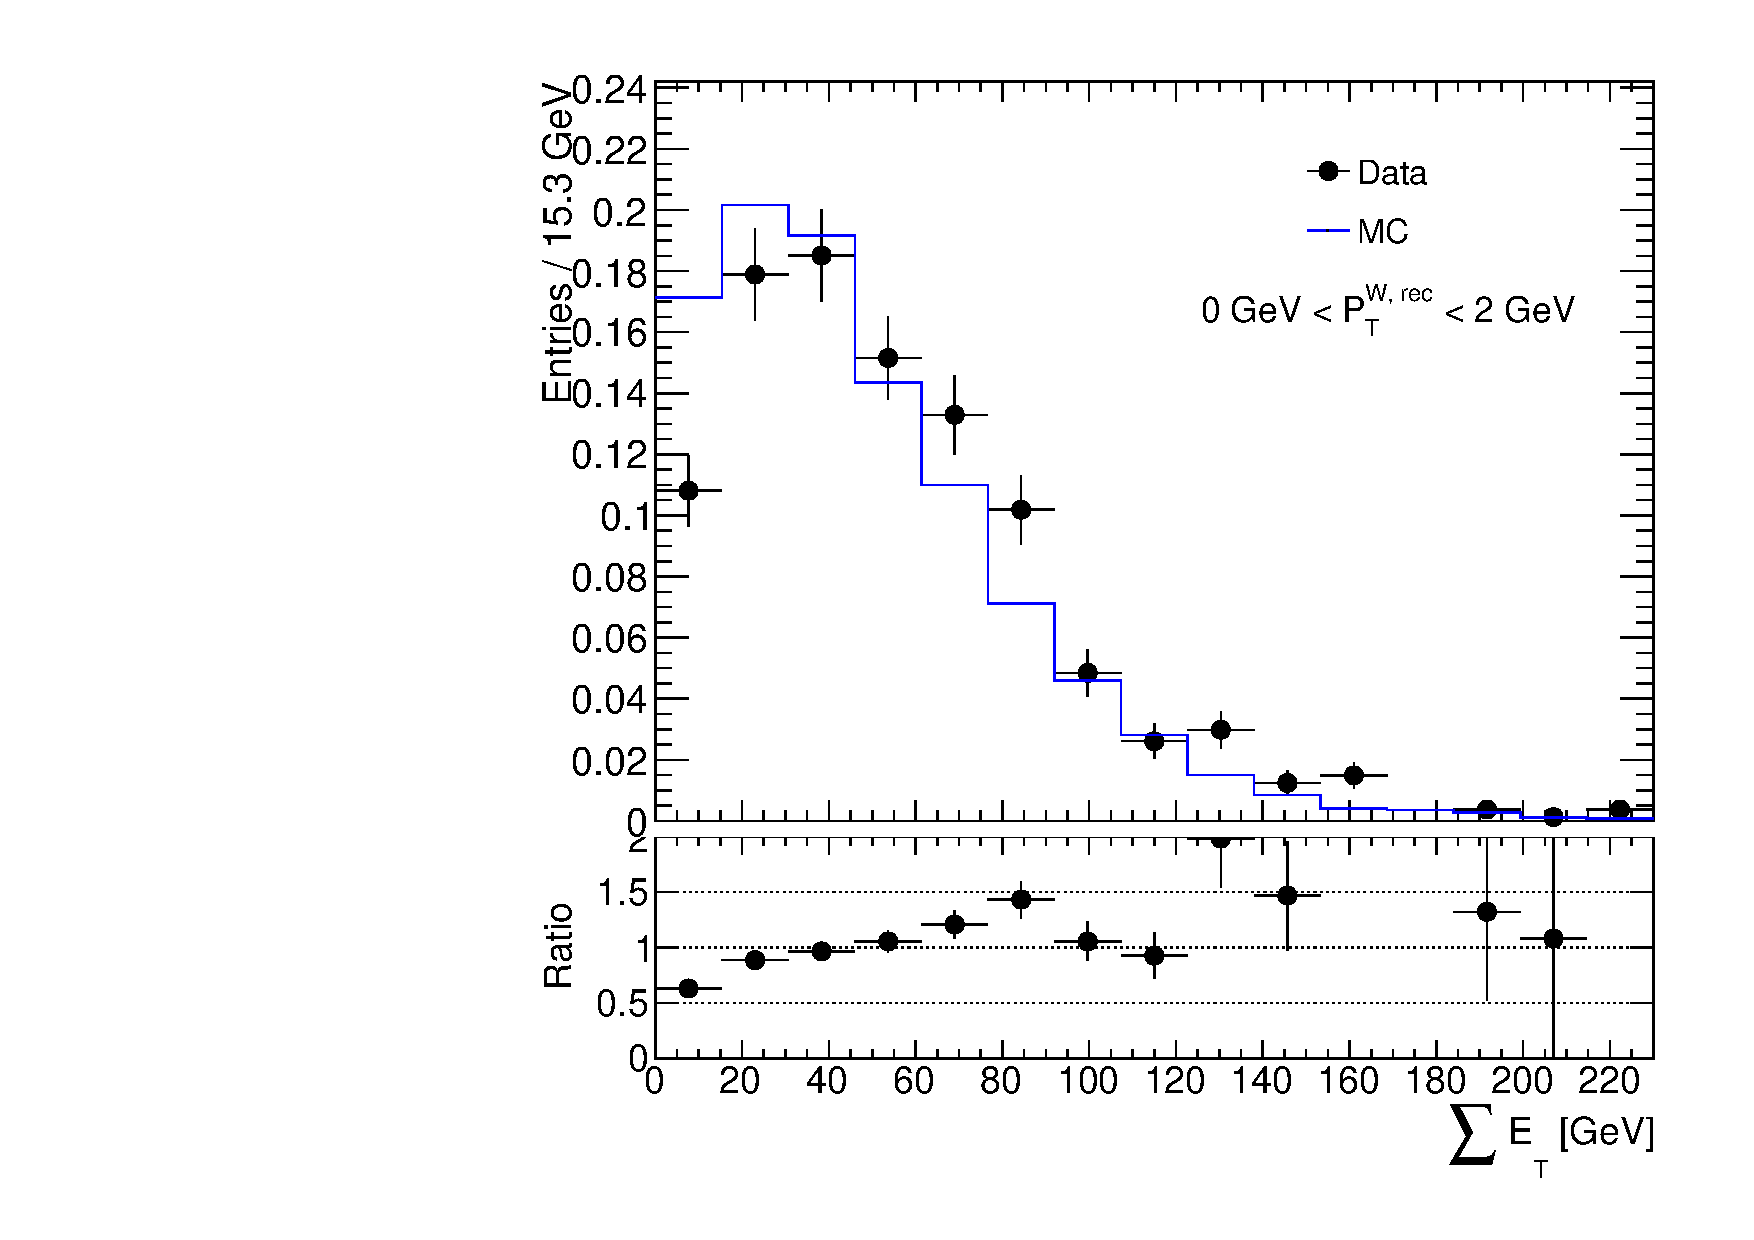
\includegraphics[width=1.\linewidth]{HadronRecoil/2.pdf} \\ a)}
\end{minipage}
\hfill
\begin{minipage}[h]{0.49\linewidth}
\center{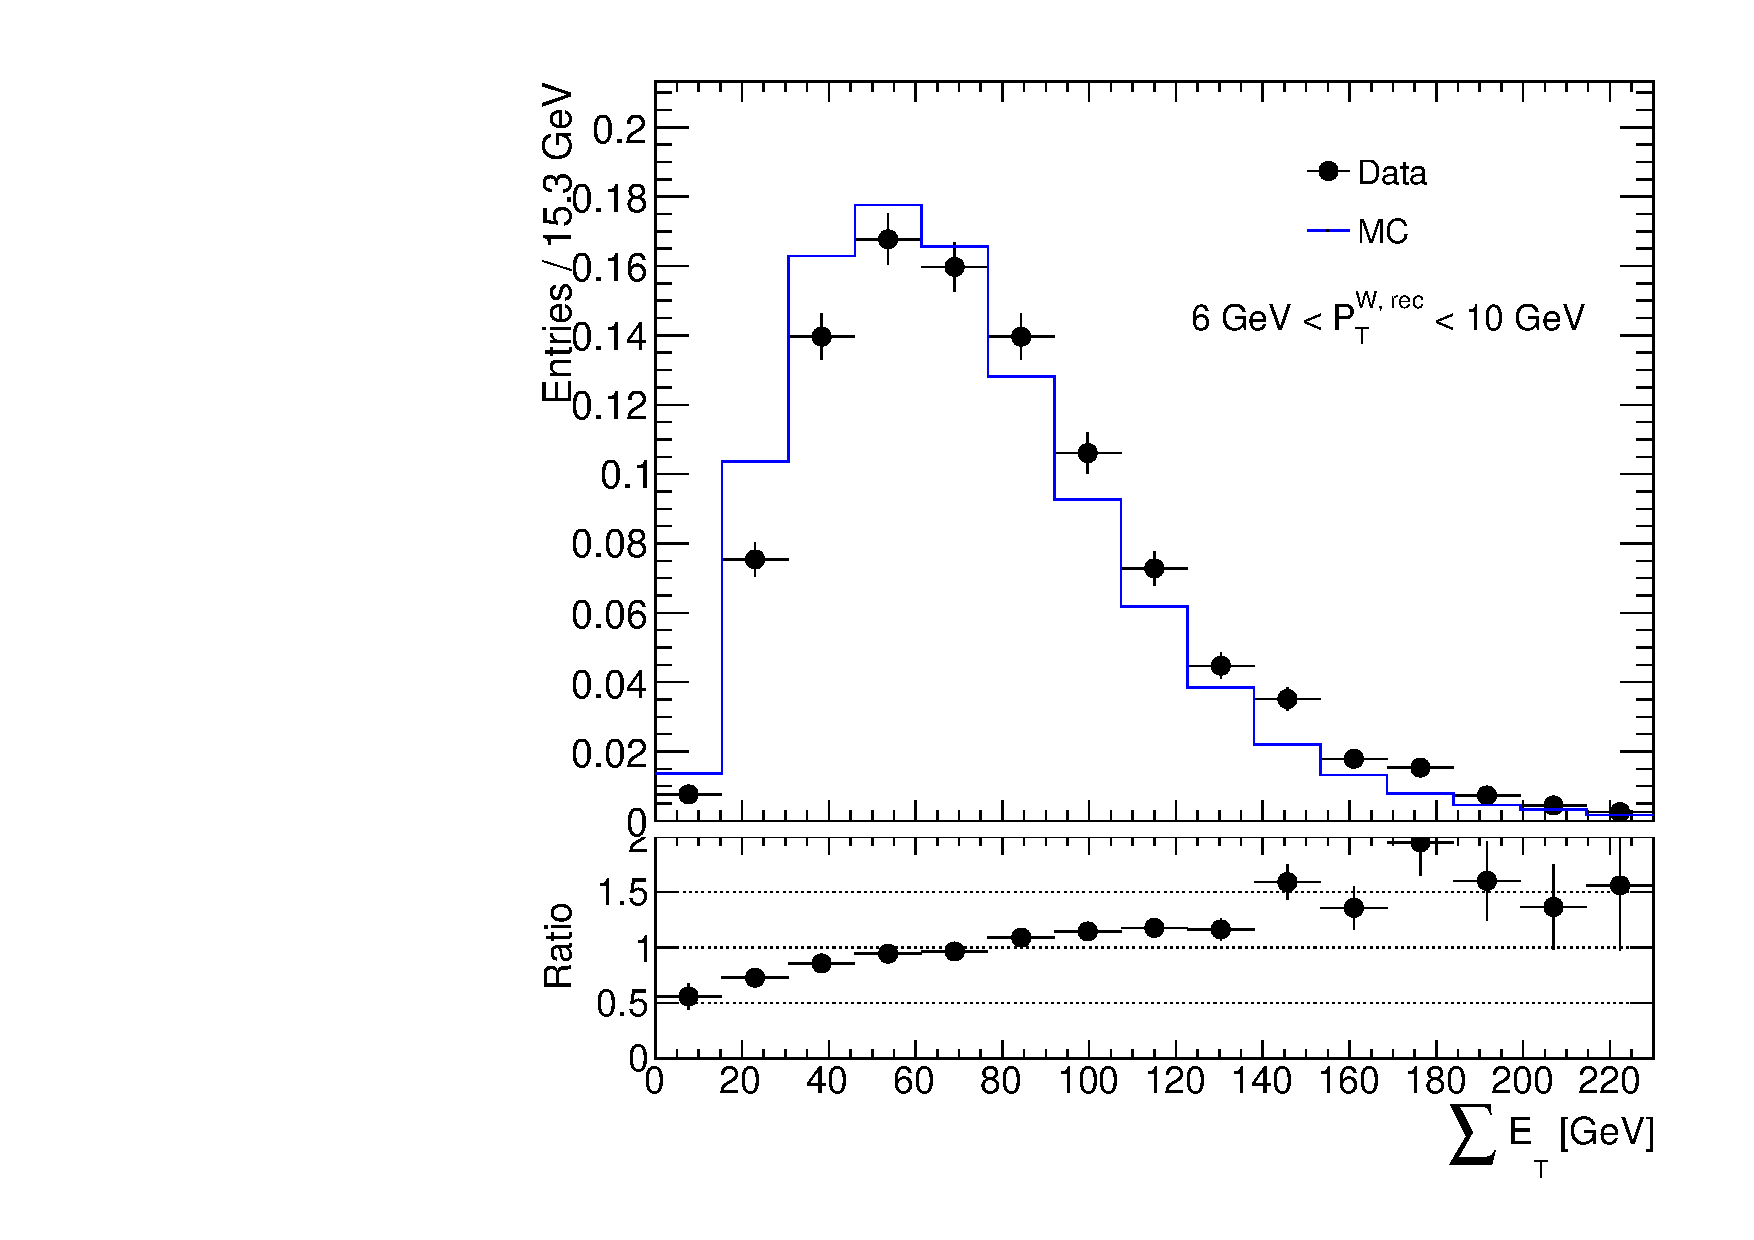
\includegraphics[width=1.\linewidth]{HadronRecoil/10.pdf} \\ b)}
\end{minipage}
\caption{Distribution of \sumet for different $p_T^{W, rec}$ bins}
\label{ris:SumEtCorPtW}
\end{figure}

\begin{figure}[!tbp]
\centering
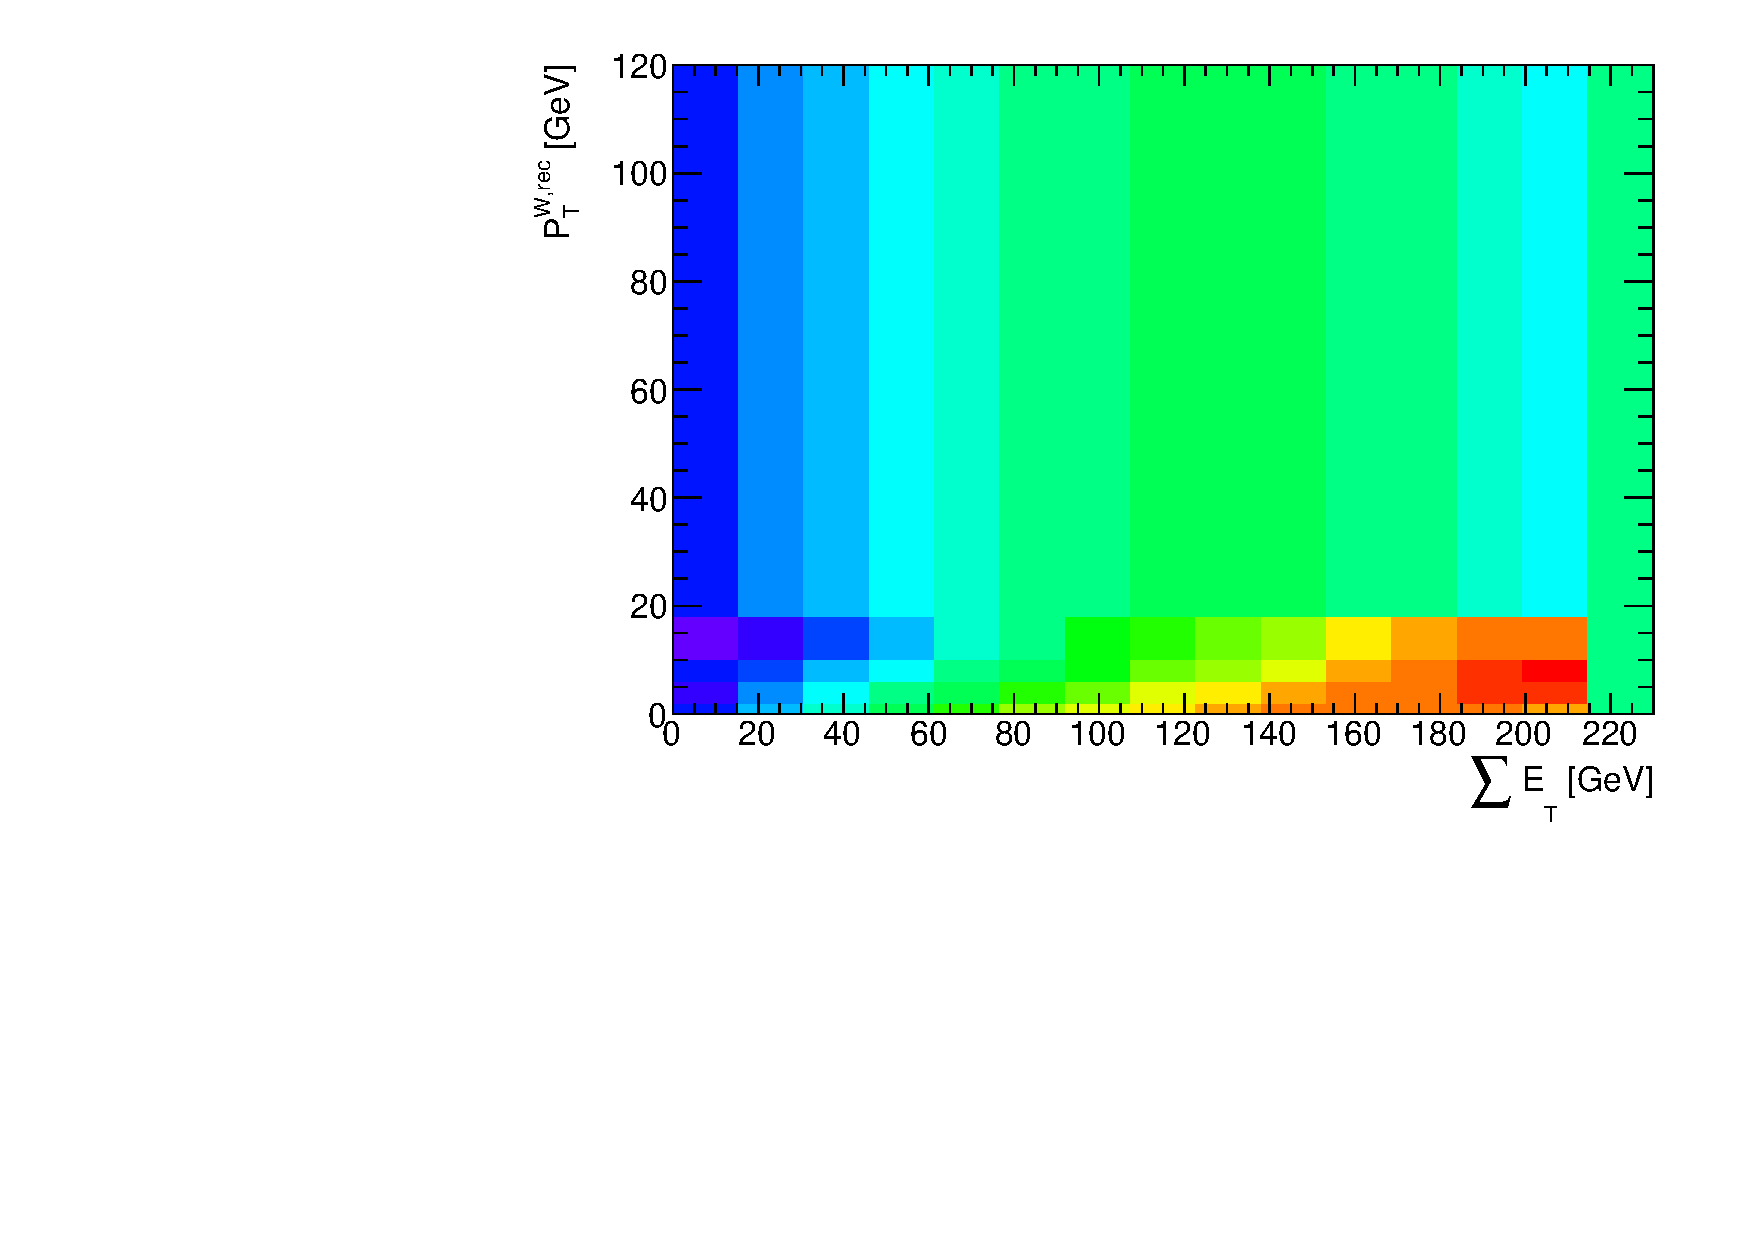
\includegraphics[width=0.7\textwidth]{HadronRecoil/SF_EP.pdf}
\caption{Correction factors for \wenu}
\label{SFWplusenu}
\end{figure}

\begin{figure}[!tbp]
\begin{minipage}[h]{0.49\linewidth}
\center{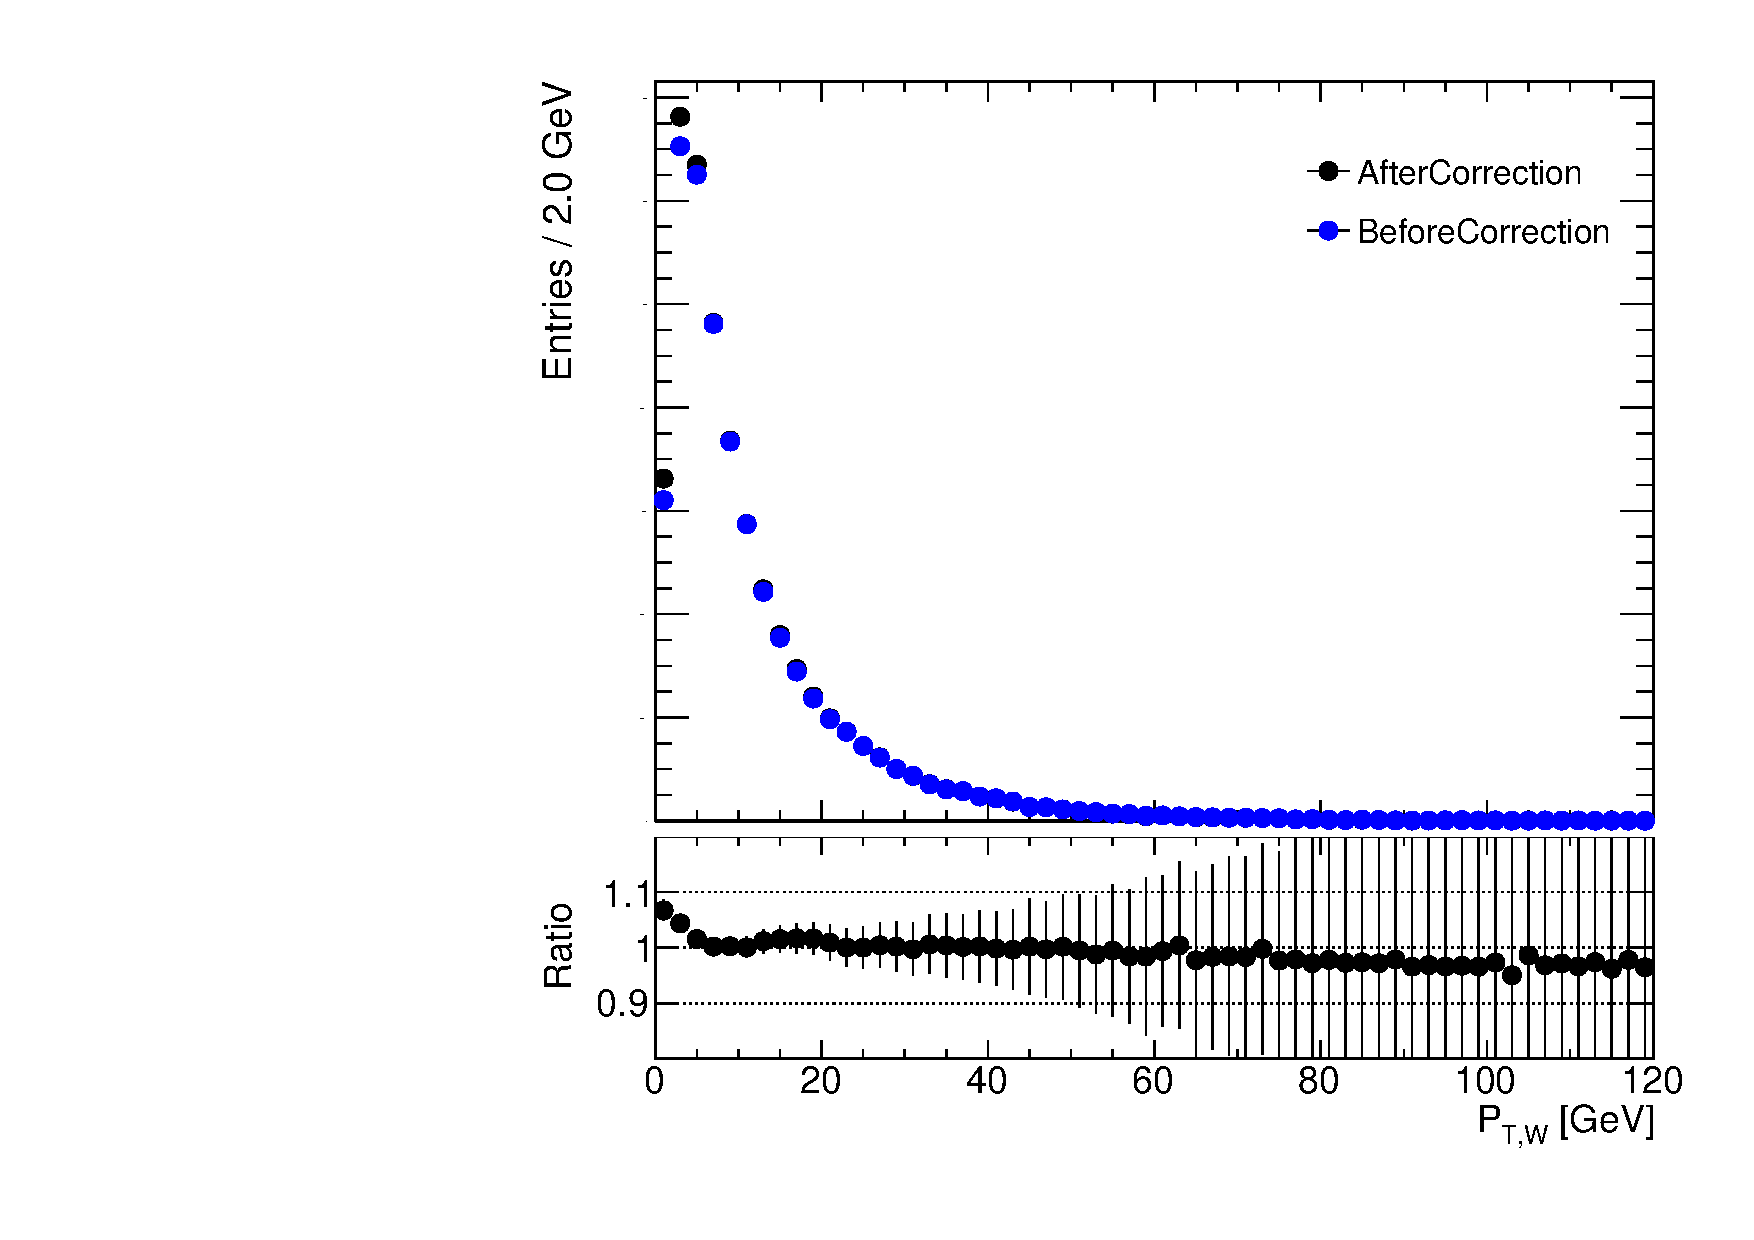
\includegraphics[width=1.\linewidth]{HadronRecoil/Wplusenu.pdf} \\ a)}
\end{minipage}
\hfill
\begin{minipage}[h]{0.49\linewidth}
\center{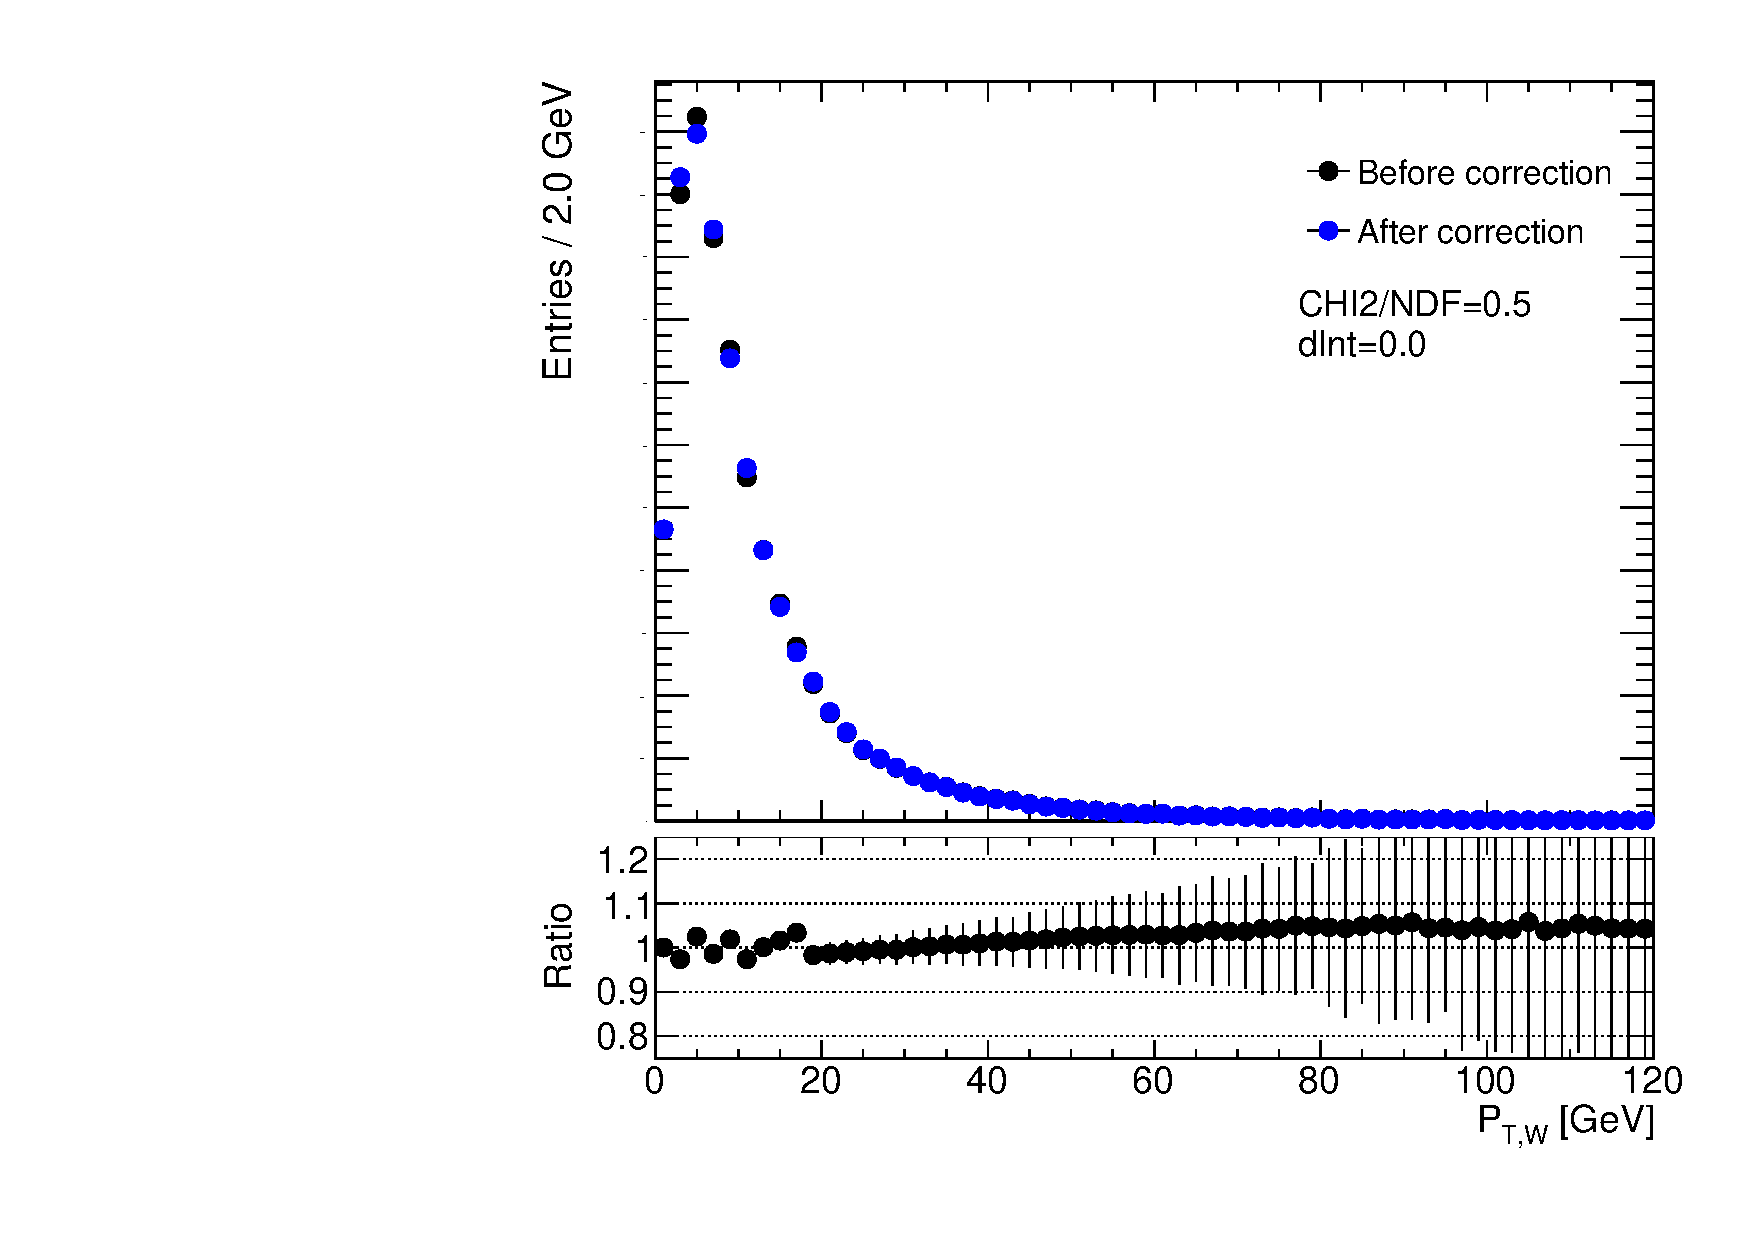
\includegraphics[width=1.\linewidth]{HadronRecoil/WplusenuRecoEffect.pdf} \\ b)}
\end{minipage}
\caption{}
\label{HadrRecoil:PtSpectrum}
\end{figure}

Statistical error of this fluctuations can be estimated from polynomial  obtained from fit using bootstrap method. Inside each bin parameters are varied within its fit uncertanty as:
\begin{equation}
fit\, parameters_{new} = fit\, parameters + gaus^{2D}(cov.matrix),
\end{equation}
where $fit\, parameters$  is a vector of best fit parameters and $gaus^{3D}$ is a 3D gaus, that takes covariance matrix from fit results. This method is allowing to take into account correlations between parameters. This procedure is repeated 25 times for each bin, that gives us set of 25 scale factors, that are later used for error determination.

Sytematical error can be studied by applying lower order of approximation on a SF or not applying it at all. The overall effect on a \cw for a different methods is shown in a Tab. \ref{SumetCW}. Results are dominated by a systematics error. However, there is a difference in a sign of the effect for a different flavors of the analysis. This cannot be explained from a physical point of view, so it was decided not to use this corrections in a final analysis.

 \begin{table}
 \caption{Effect of \sumet correction on a $C_{W}$ for a different channels and methods}
\label{SumetCW}
\begin{center}
\begin{tabular}{c | c |  c |  c   }
\hline
Channel & $\delta C_W$ & $\delta C_W$ & $\delta C_W$ \\
& polynomial order 2 & polynomial order 1 & Toy MC \\
\hline
\hline
$W^{+} \to e^{+}\nu$ & 0.39\%  & 0.31\% & 0.03\% \\
$W^{-} \to e^{-}\nu$ & 0.33\%  & 0.22\% & 0.03\% \\
$W^{+} \to \mu^{+}\nu$ & -0.20\%  & -0.28\% & 0.03\% \\
$W^{-} \to \mu^{-}\nu$ & -0.21\%  & -0.27\% & 0.03\% \\
\hline
\end{tabular}
\end{center}

\end{table}


\subsection{Resolution correction using Z events}
Another way to check resolution effects is to use \uperp and \upar  $ - p_T^{Z}$ distributions in a Z events. This correction assumes, that any resolution mismodelling reflects discrepancies in the \sumet distribution, while difference in resolution at a given \sumet is a subleading. There is a clear difference in a rms of this distributions between data and MC, that cannot be accounted as a statistical error in data. Difference in resolutions is consistent for \uperp and \upar $- p_T^{Z}$ distributions, but depends on a flavor of the analysis.  The resolution is corrected by smearing with a Gaussian distribution each component of a hadron recoil:

\begin{figure}[!tbp]
\begin{minipage}[h]{0.40\linewidth}
\center{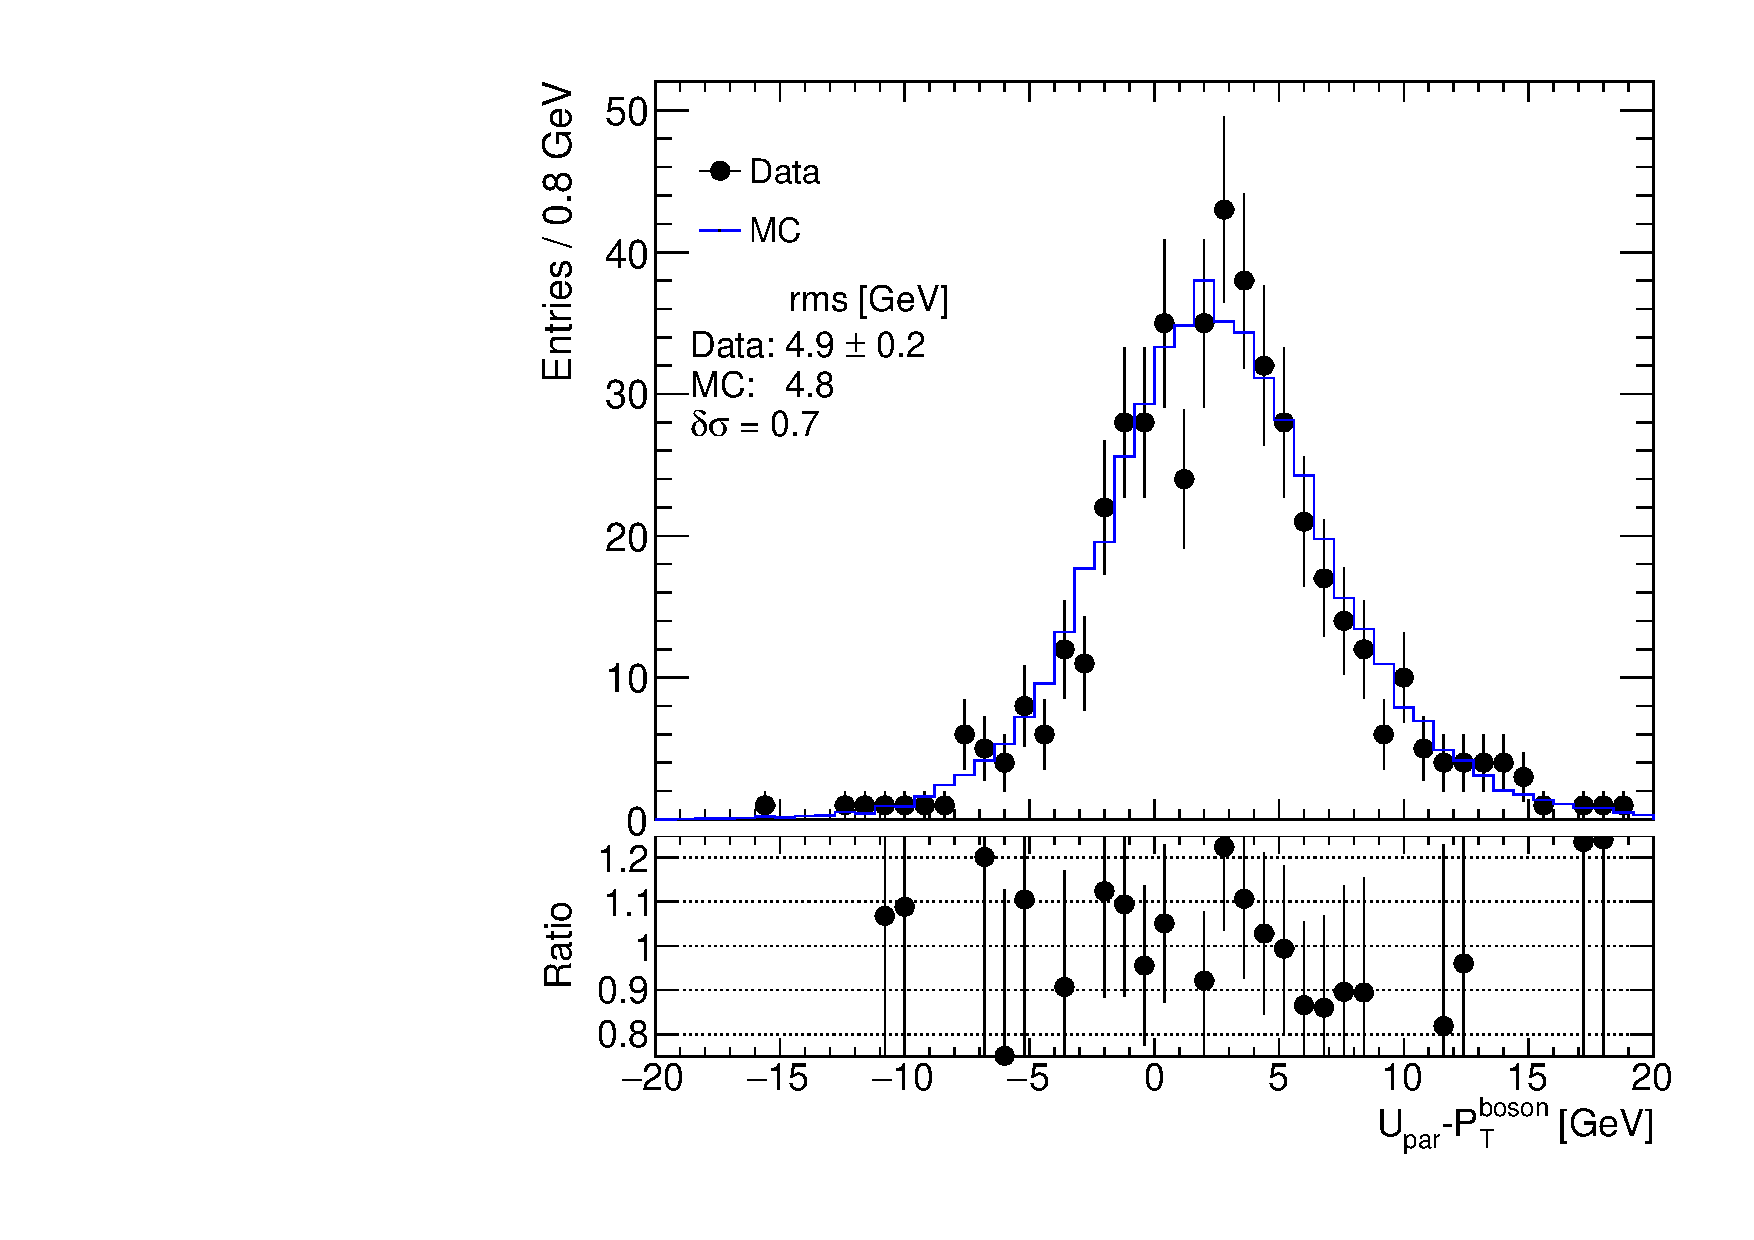
\includegraphics[width=1.\linewidth]{HadronRecoil/UParERMS.pdf} \\ a)}
\end{minipage}
\hfill
\begin{minipage}[h]{0.40\linewidth}
\center{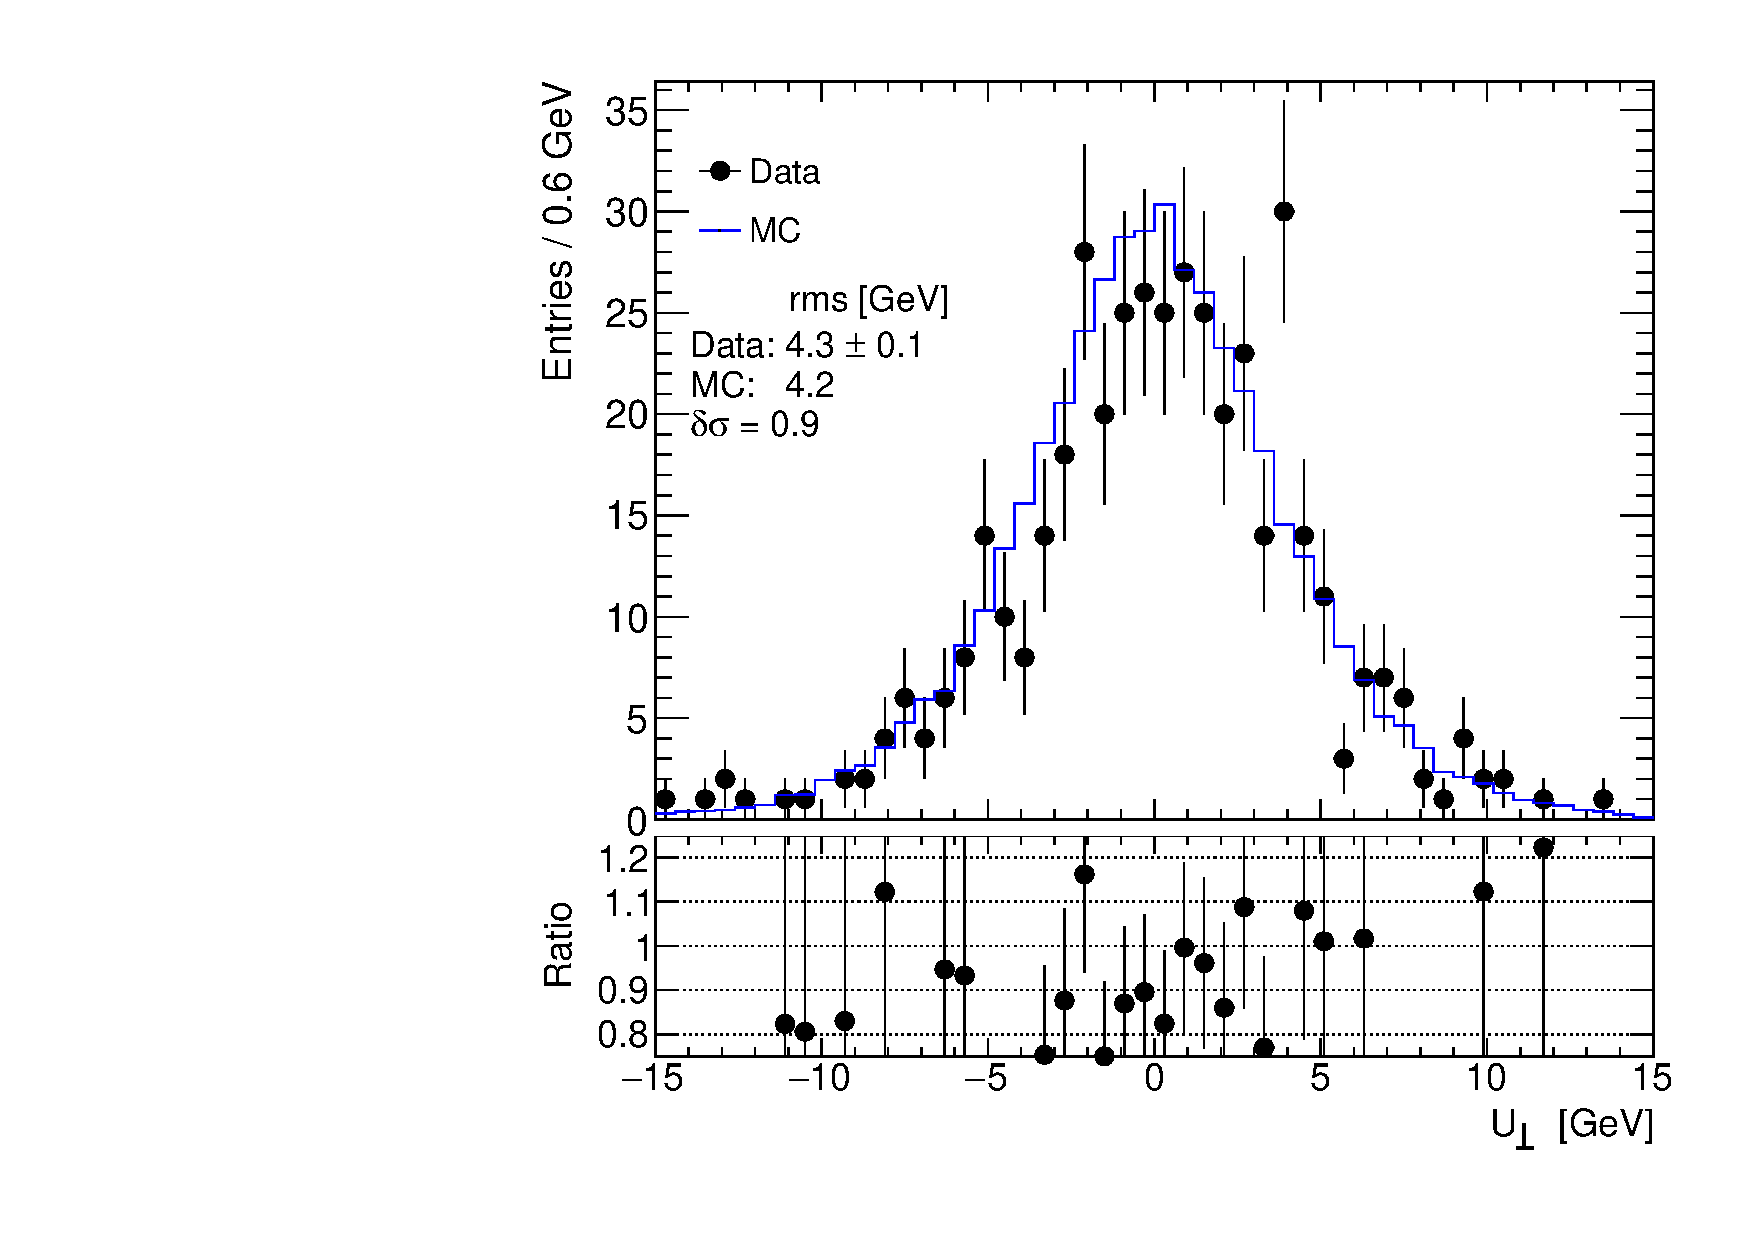
\includegraphics[width=1.\linewidth]{HadronRecoil/UPerpERMS.pdf} \\ b)}
\end{minipage}
\vfill
\begin{minipage}[h]{0.40\linewidth}
\center{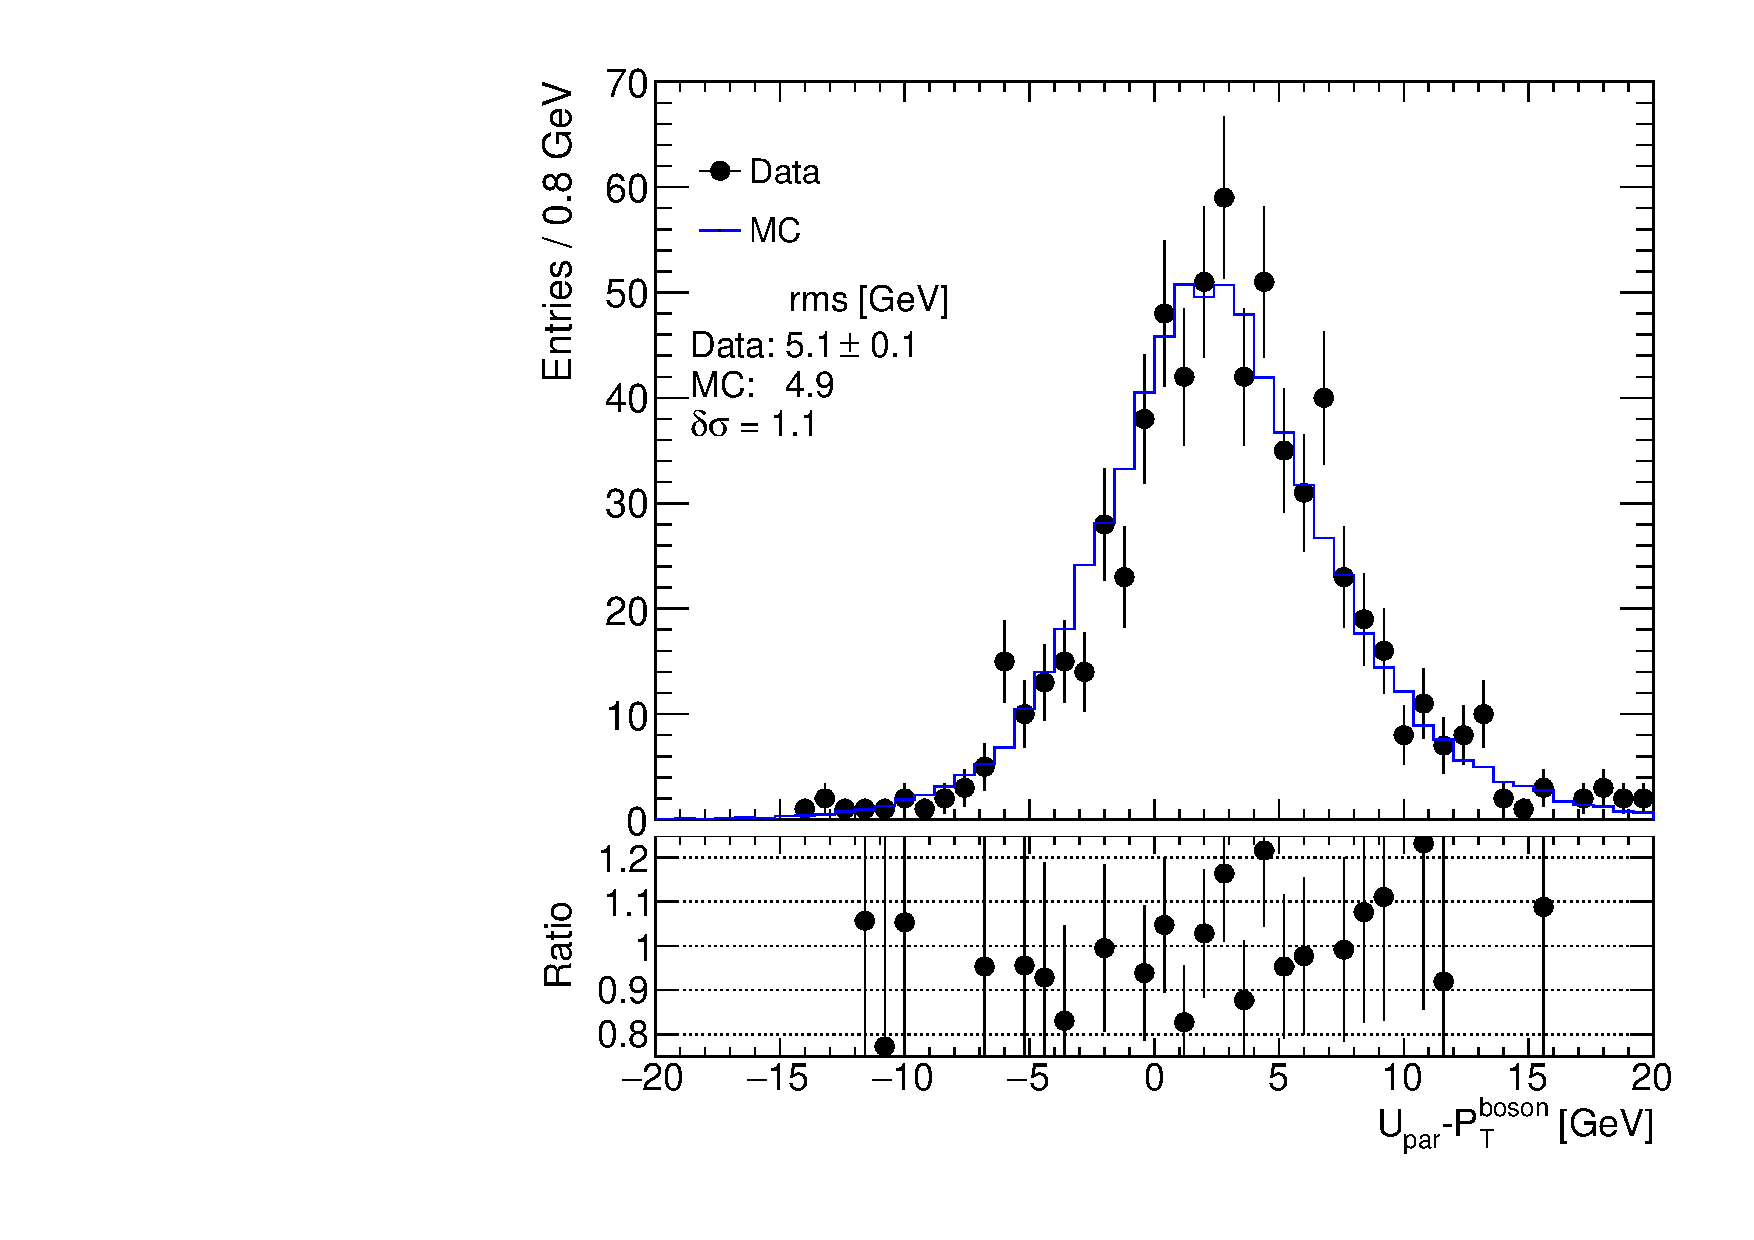
\includegraphics[width=1.\linewidth]{HadronRecoil/UParMRMS.pdf} \\ a)}
\end{minipage}
\hfill
\begin{minipage}[h]{0.40\linewidth}
\center{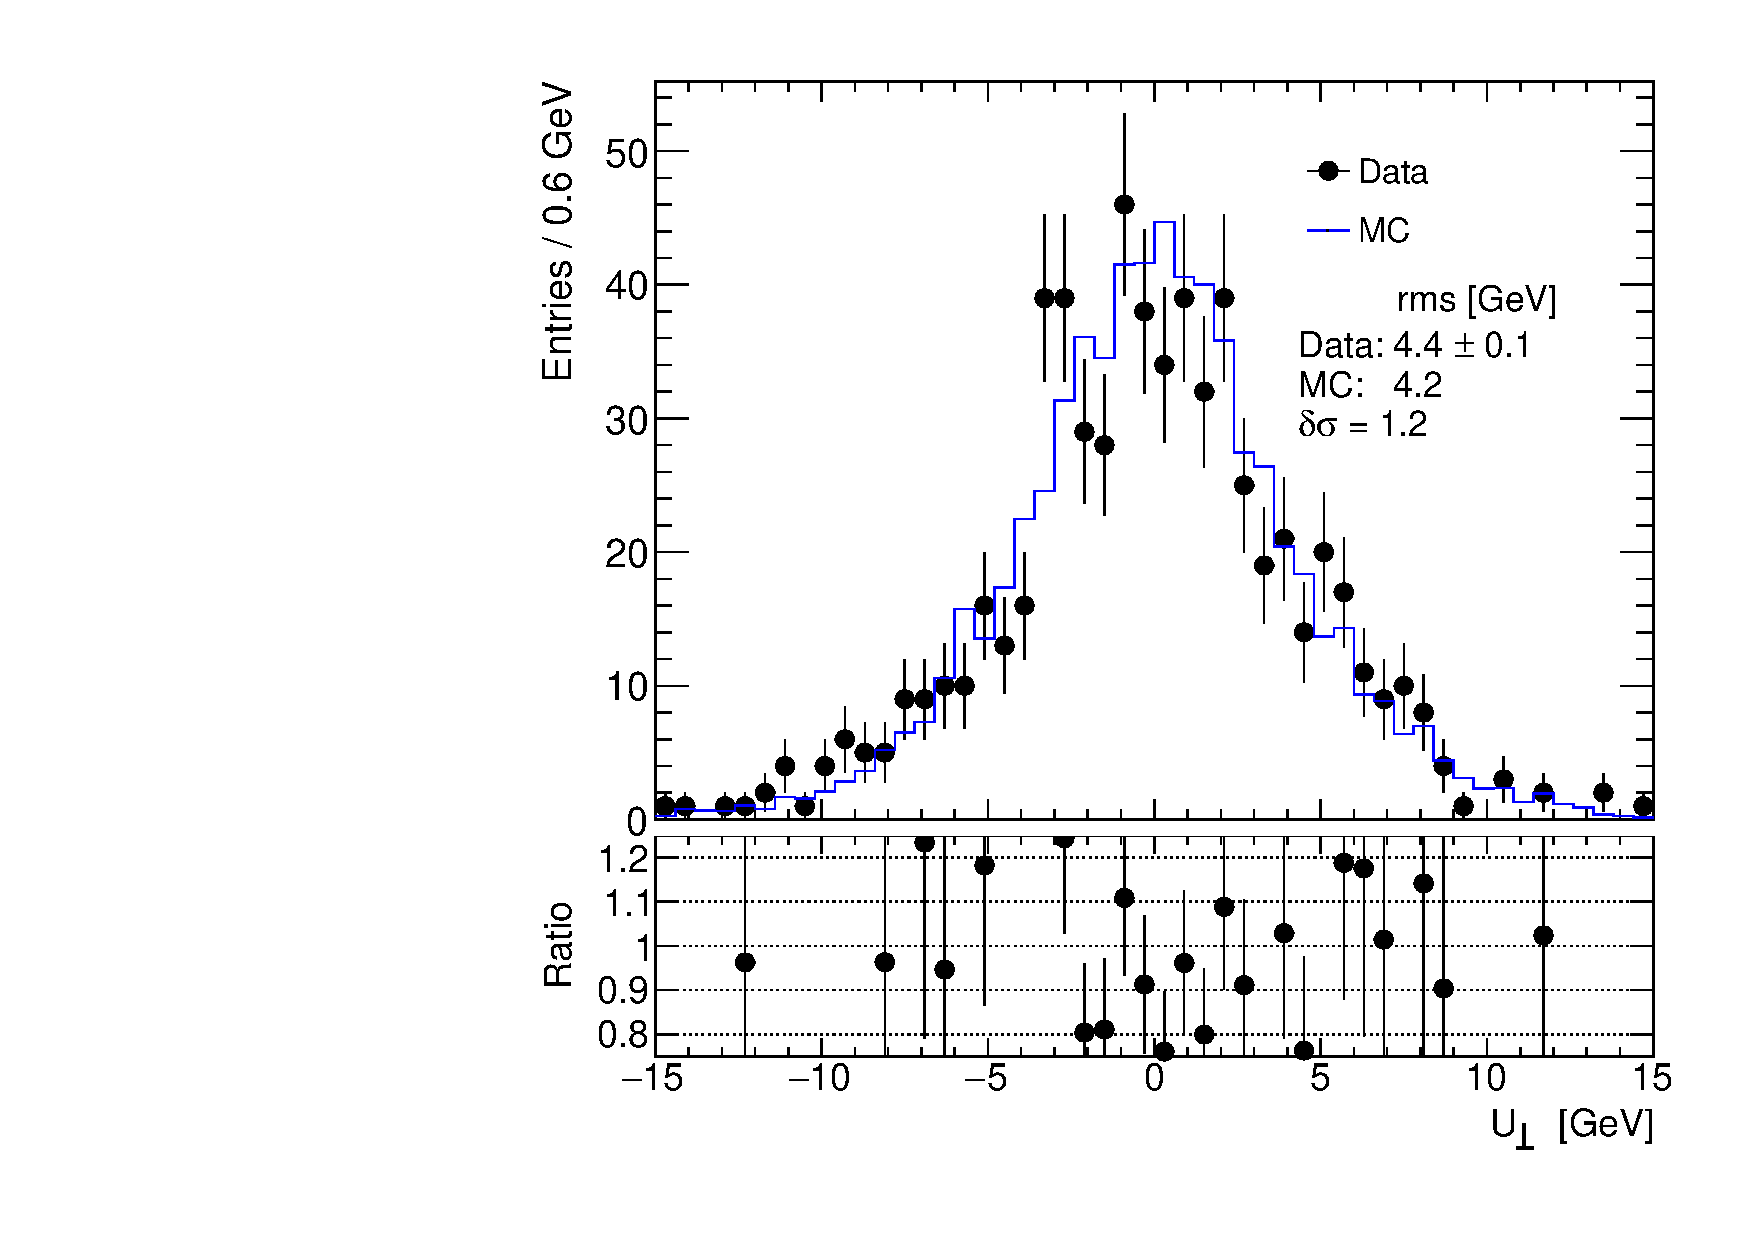
\includegraphics[width=1.\linewidth]{HadronRecoil/UPerpMRMS.pdf} \\ b)}
\end{minipage}
\vfill
\begin{minipage}[h]{0.40\linewidth}
\center{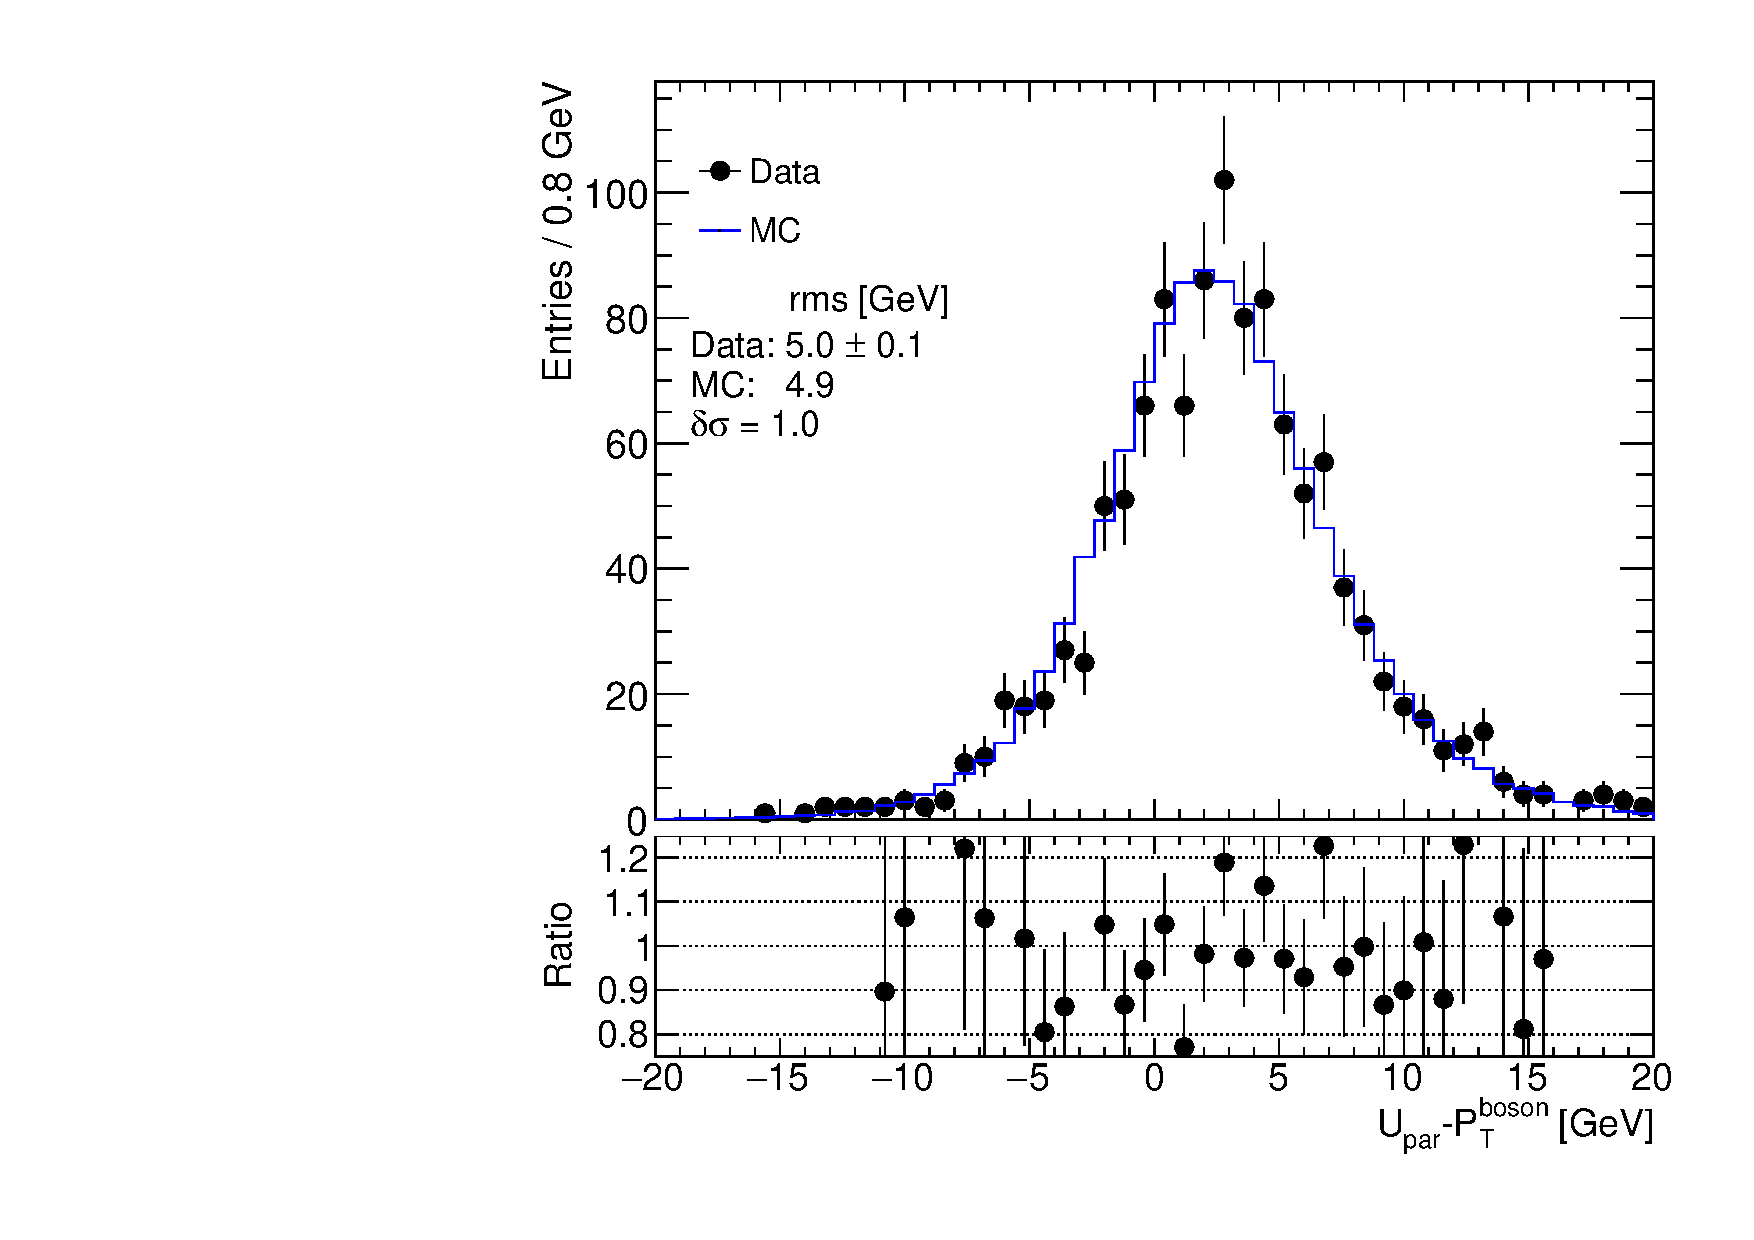
\includegraphics[width=1.\linewidth]{HadronRecoil/UParTotalRMS.pdf} \\ a)}
\end{minipage}
\hfill
\begin{minipage}[h]{0.40\linewidth}
\center{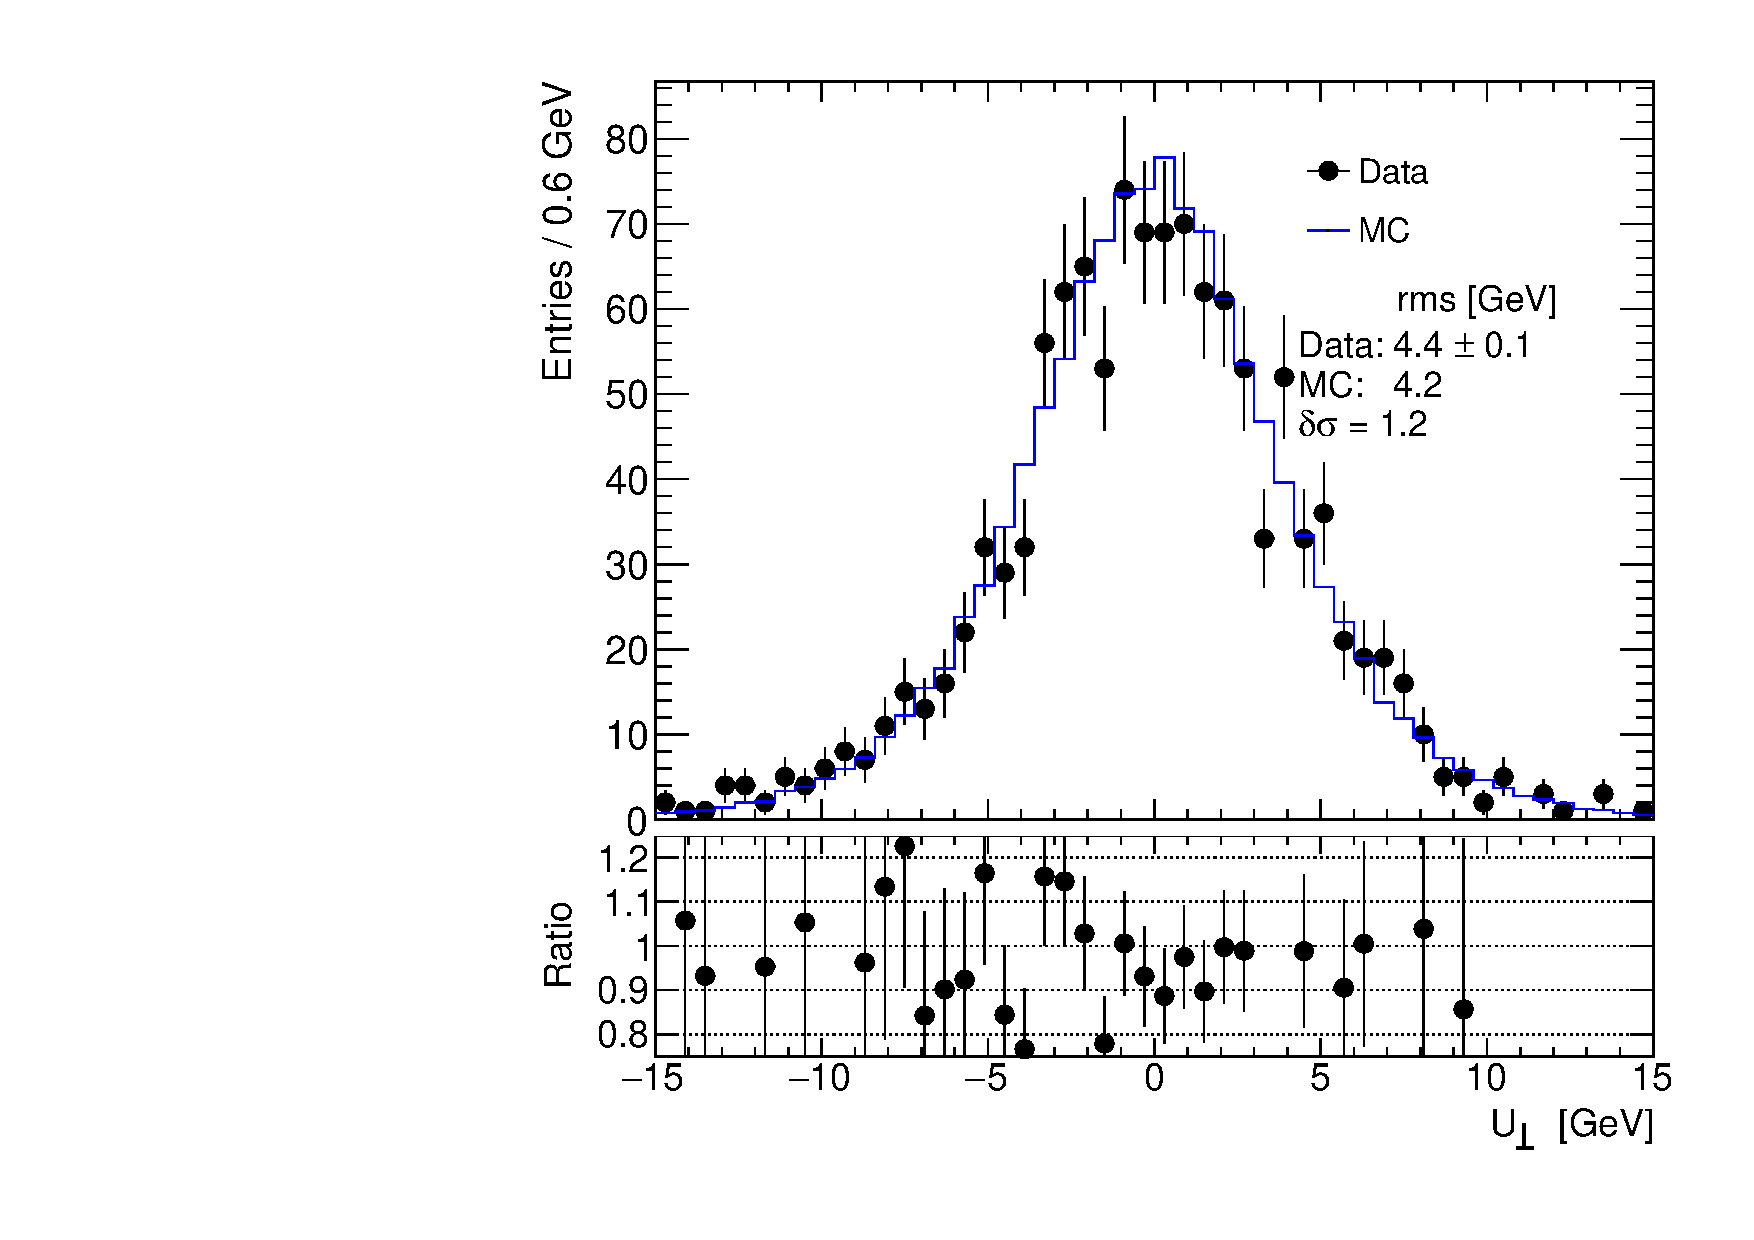
\includegraphics[width=1.\linewidth]{HadronRecoil/UPerpTotalRMS.pdf} \\ b)}
\end{minipage}
\caption{}
\label{HadrRecoil:CorrSumet}
\end{figure}

\begin{equation}
\upar' = \upar+Gaus(0, d\sigma)
\end{equation}
\begin{equation}
\uperp' = \uperp + Gaus(0, d\sigma),
\end{equation}
where $d\sigma$ is a difference in a resoultions calculated as:
\begin{equation}
d\sigma=\sqrt{\sigma_{data}^2-\sigma_{MC}^2}
\end{equation}
Systematic error of this $d\sigma$ is taken as an statistical error for $\sigma_{data}$. Overall effect on a \cw depending on a $d\sigma$ is shown on a Fig. \ref{ris:CwSmear}.
Due to a random nature of this correction, effect is not stable for a small $d\sigma$. Stability of this correction can be tested by repeating this procedure several times with different random seed number. Due to a not stable nature of this correction the overall systematics coming from resolution mismodelling is assumed to be 0.2\% for each W channel.
\begin{figure}[!tbp]
\begin{minipage}[h]{0.49\linewidth}
\center{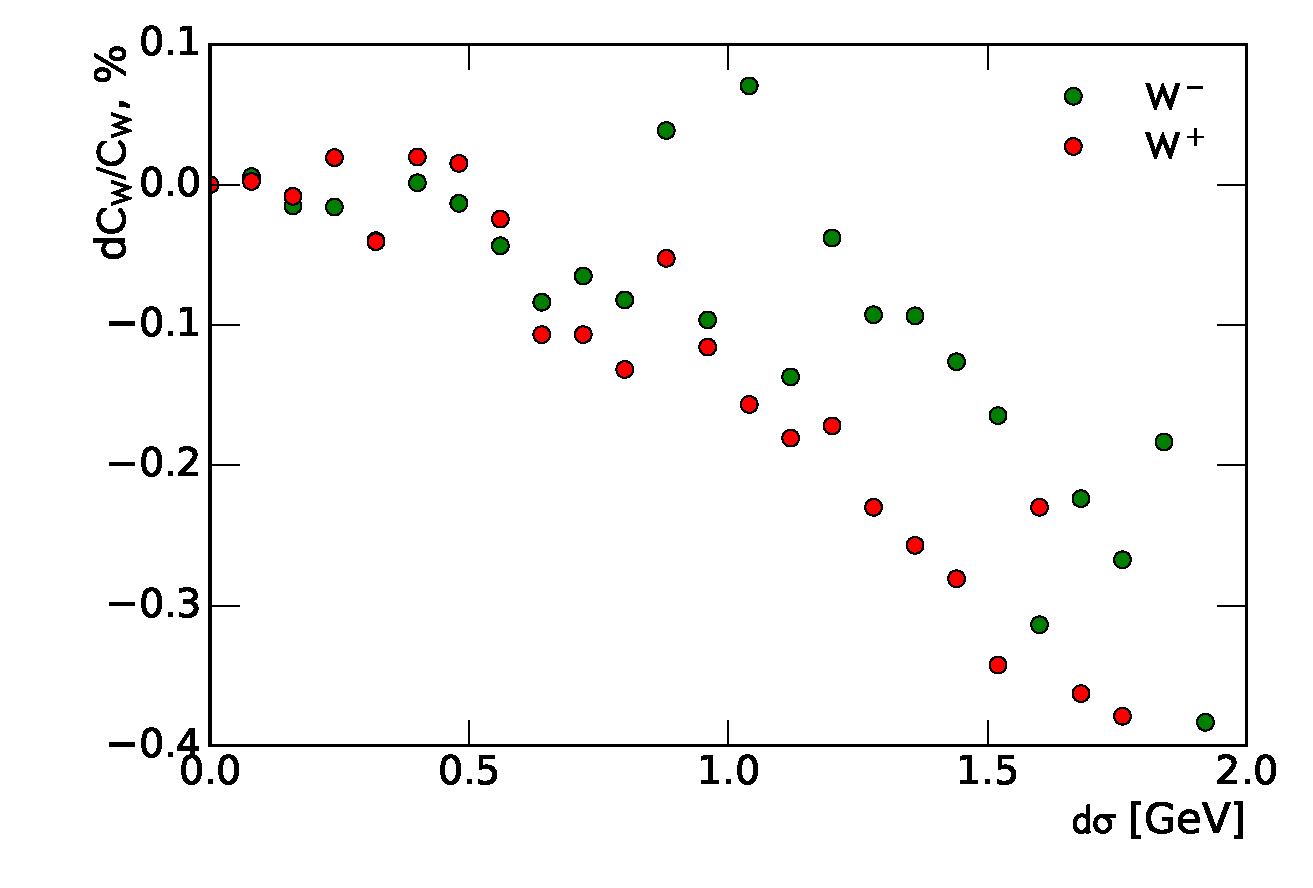
\includegraphics[width=1.\linewidth]{HadronRecoil/CWElectronSmearing.pdf} \\ a)}
\end{minipage}
\hfill
\begin{minipage}[h]{0.49\linewidth}
\center{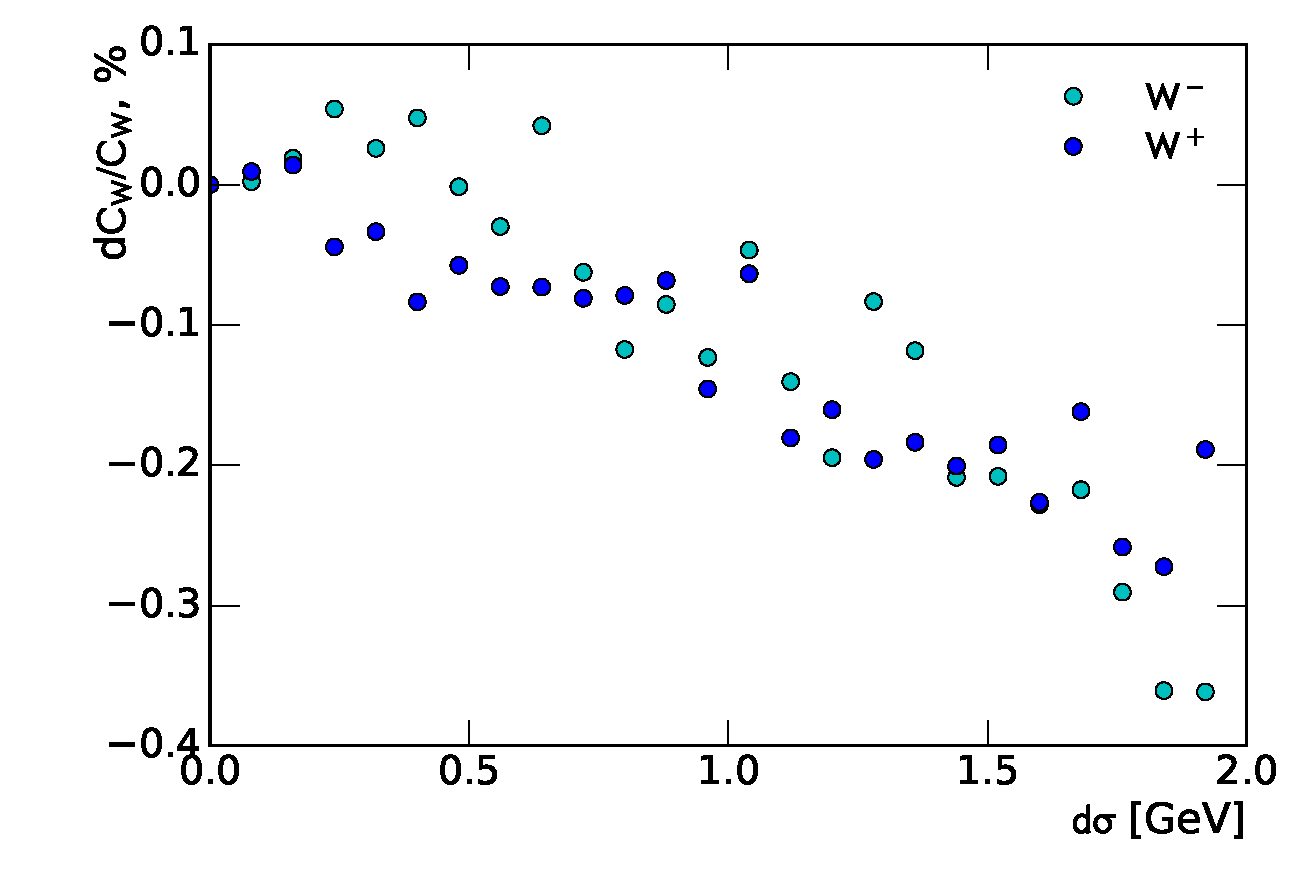
\includegraphics[width=1.\linewidth]{HadronRecoil/CWMuonSmearing.pdf} \\ b)}
\end{minipage}
\caption{Effect on a \cw for a different $d\sigma$ for a) \wenu b)\wmunu channel}
\label{ris:CwSmear}
\end{figure}


\section{Hadron recoil bias correction}

\begin{table}[!tbp]
\caption{}
\label{tab:SFHadronRecoil}
\begin{center}
\begin{tabular}{| l | c | c |}
\hline
Method & SF & error \\
\hline
\hline
Mean $M_T^{W}$ & 1.10 & 0.2\\
$M_T^{W}$ \chiD & 1.01 & 0.07 \\
\upar \chiD & 1.00 & 0.014 \\
\hline
\end{tabular}
\end{center}
\end{table}


\begin{figure}[!tbp]
\minipage{0.32\textwidth}
  \center{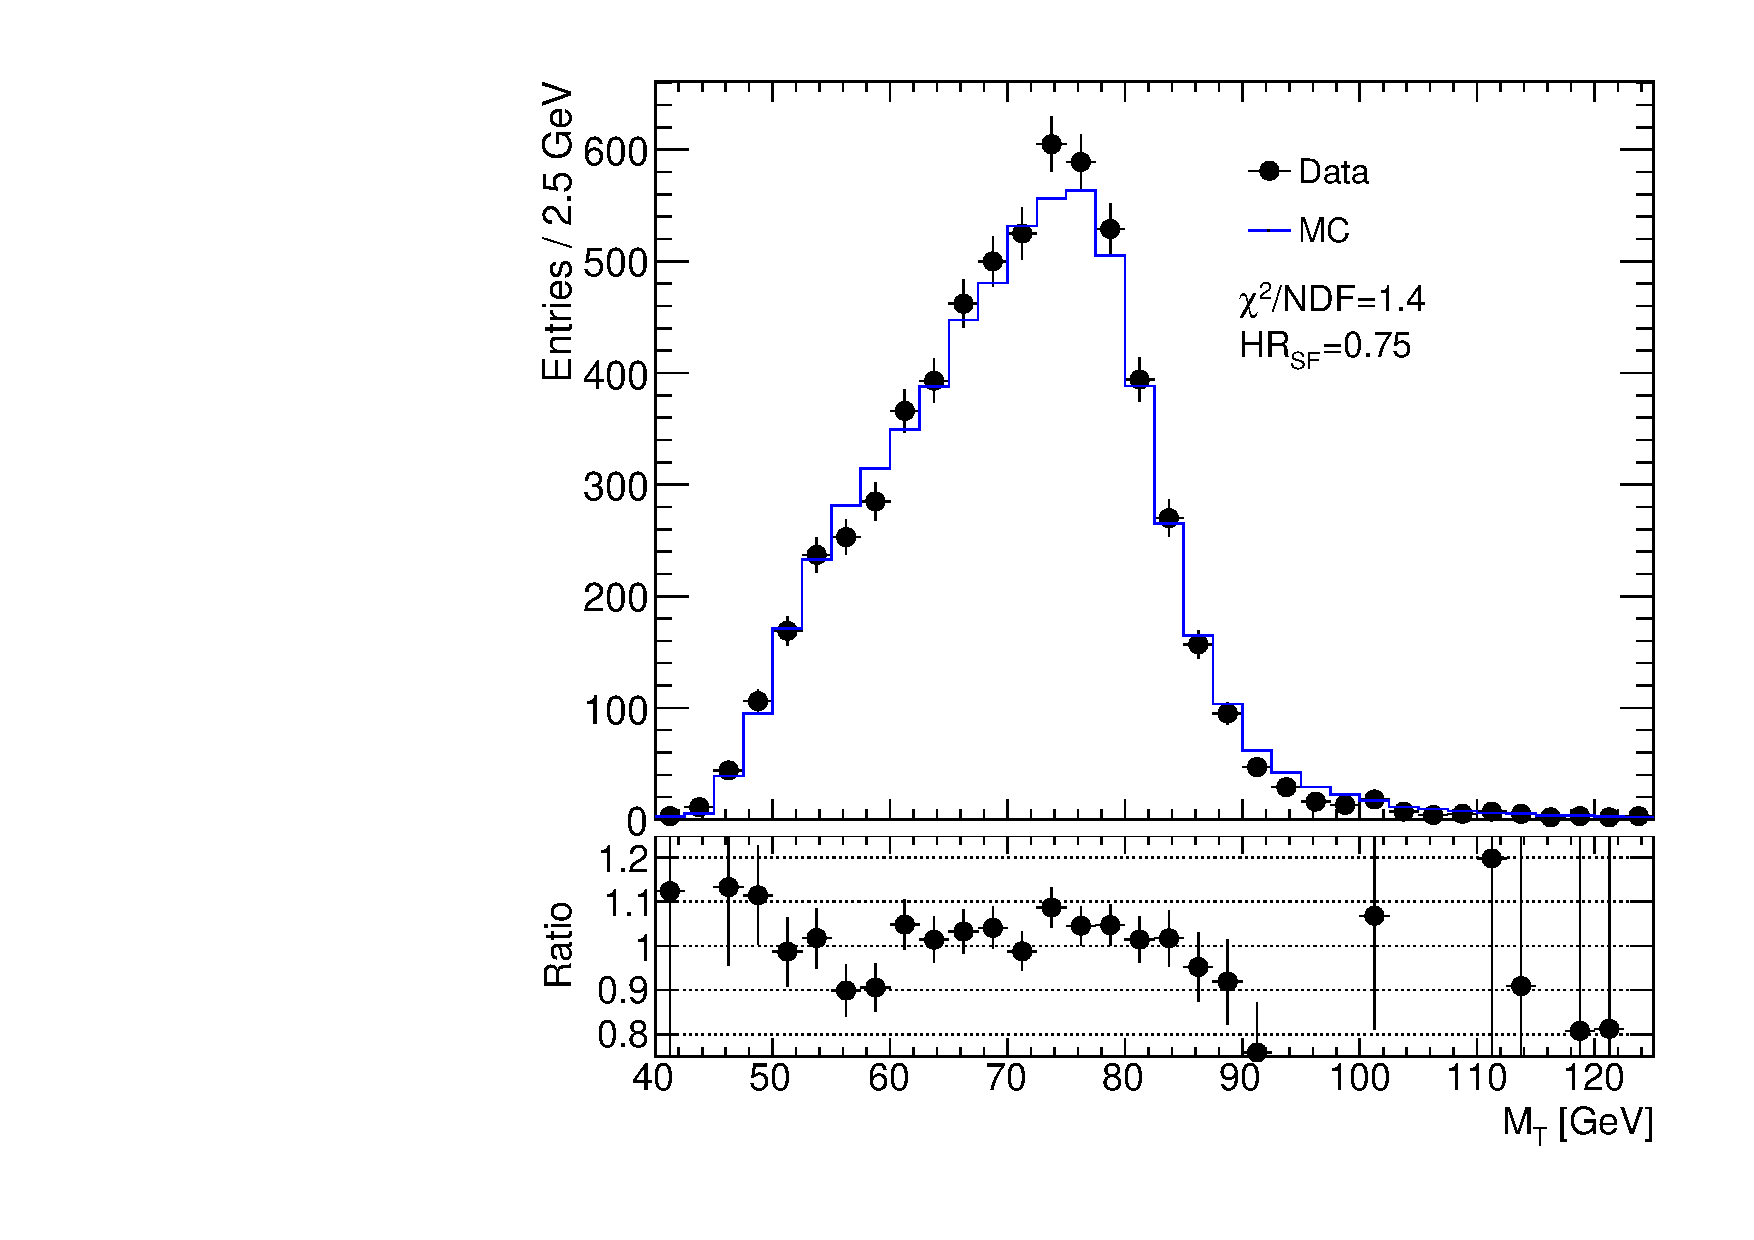
\includegraphics[width=\linewidth]{HadronRecoil/MtWEScale0.pdf} a)}
\endminipage\hfill
\minipage{0.32\textwidth}
   \center{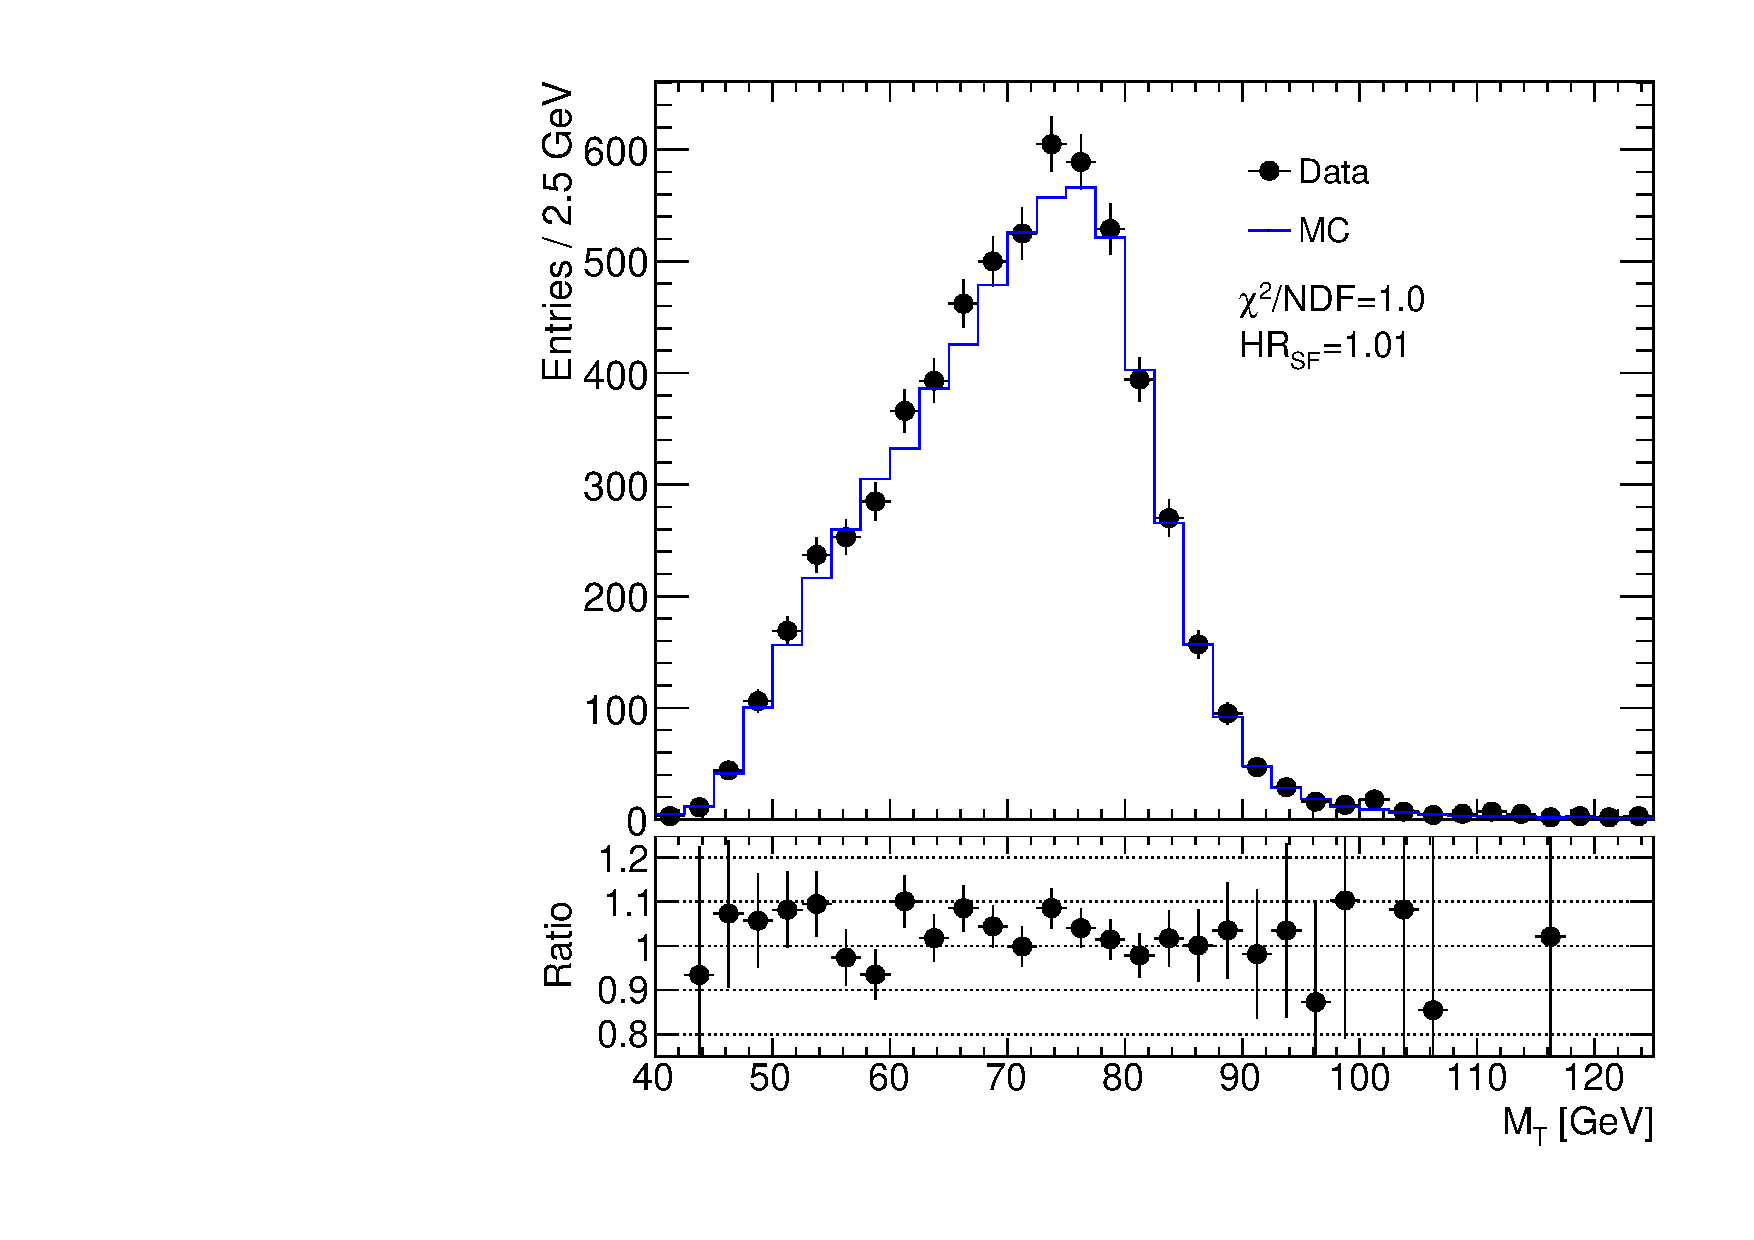
\includegraphics[width=\linewidth]{HadronRecoil/MtWEScale13.pdf} b)}
\endminipage\hfill
\minipage{0.32\textwidth}%
   \center{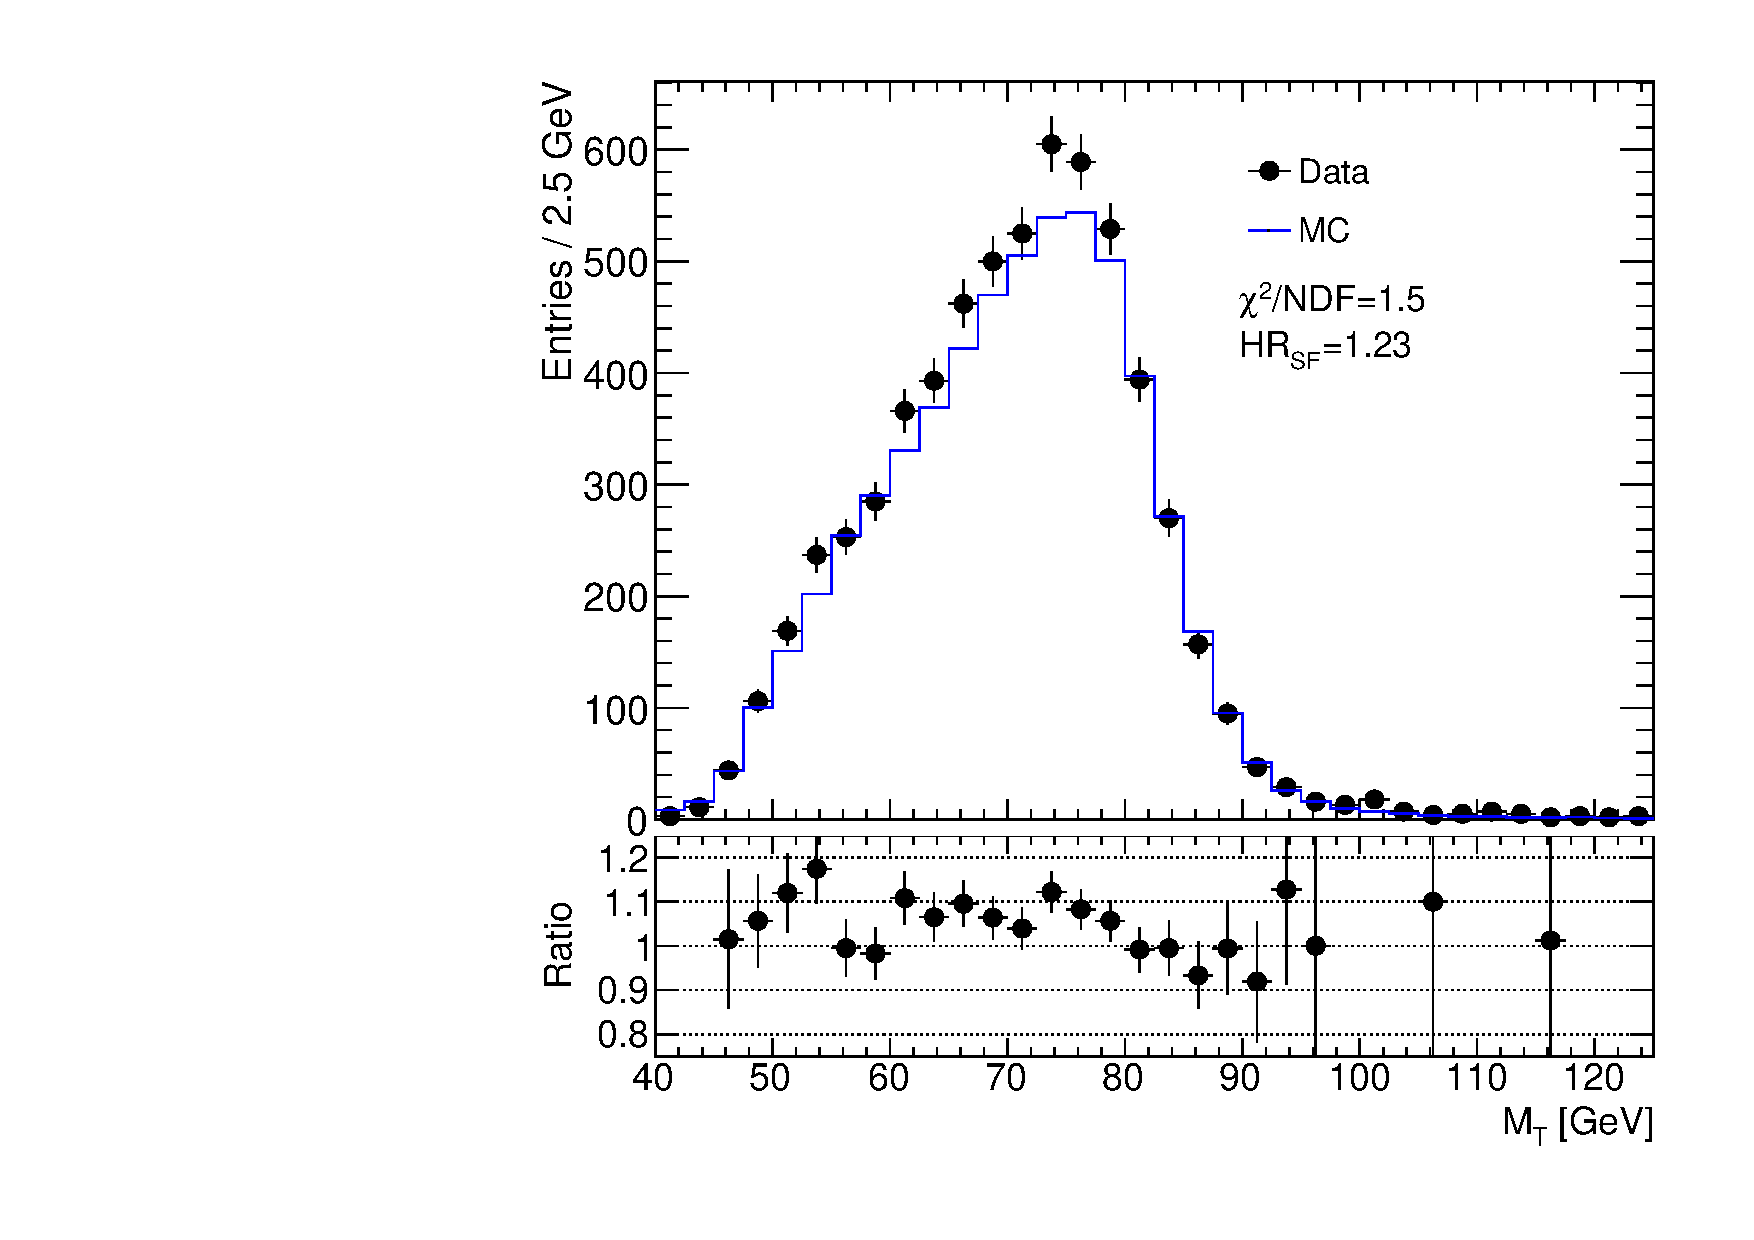
\includegraphics[width=\linewidth]{HadronRecoil/MtWEScale24.pdf} c)}
\endminipage
\caption{}
\label{HadronRecoilScaleMtW}
\vfill
\minipage{0.32\textwidth}
  \center{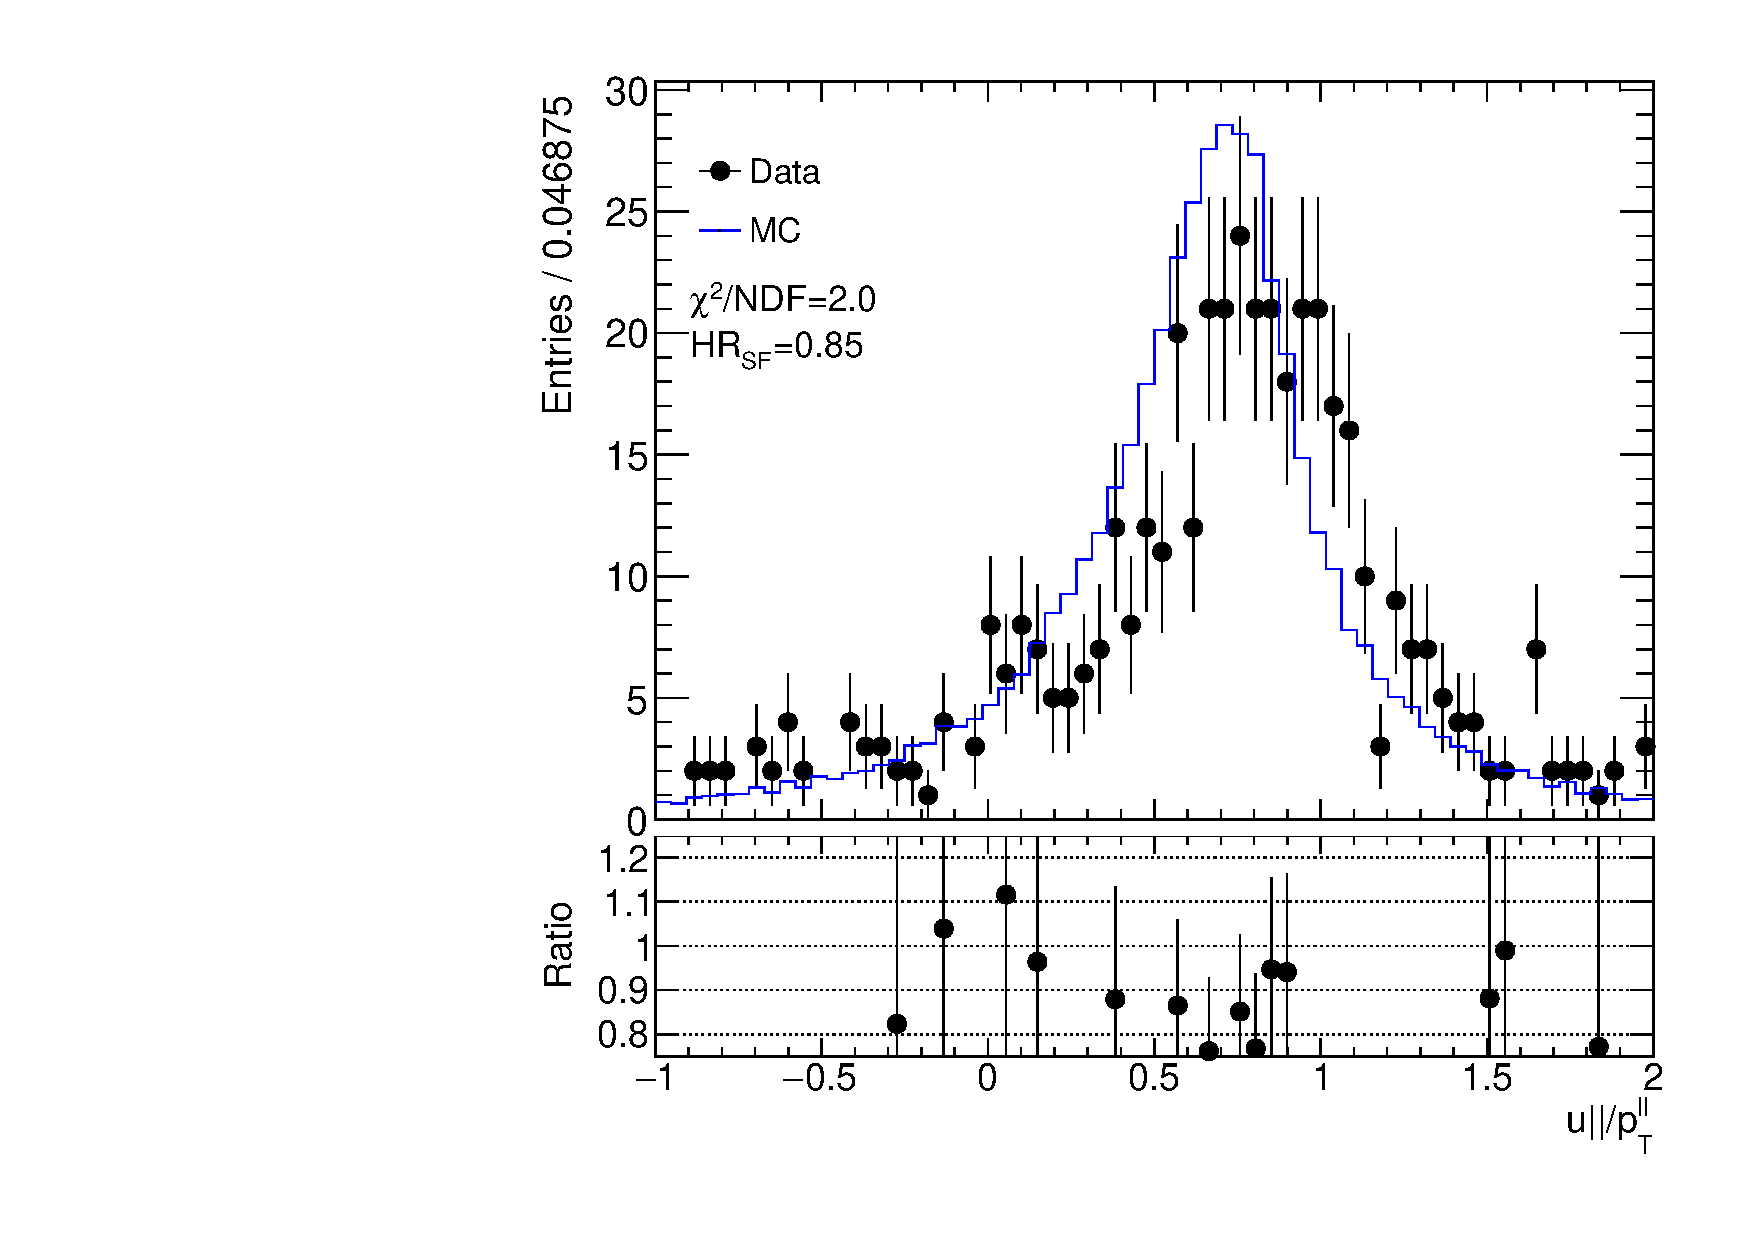
\includegraphics[width=\linewidth]{HadronRecoil/UParEScale5.pdf} a)}
\endminipage\hfill
\minipage{0.32\textwidth}
   \center{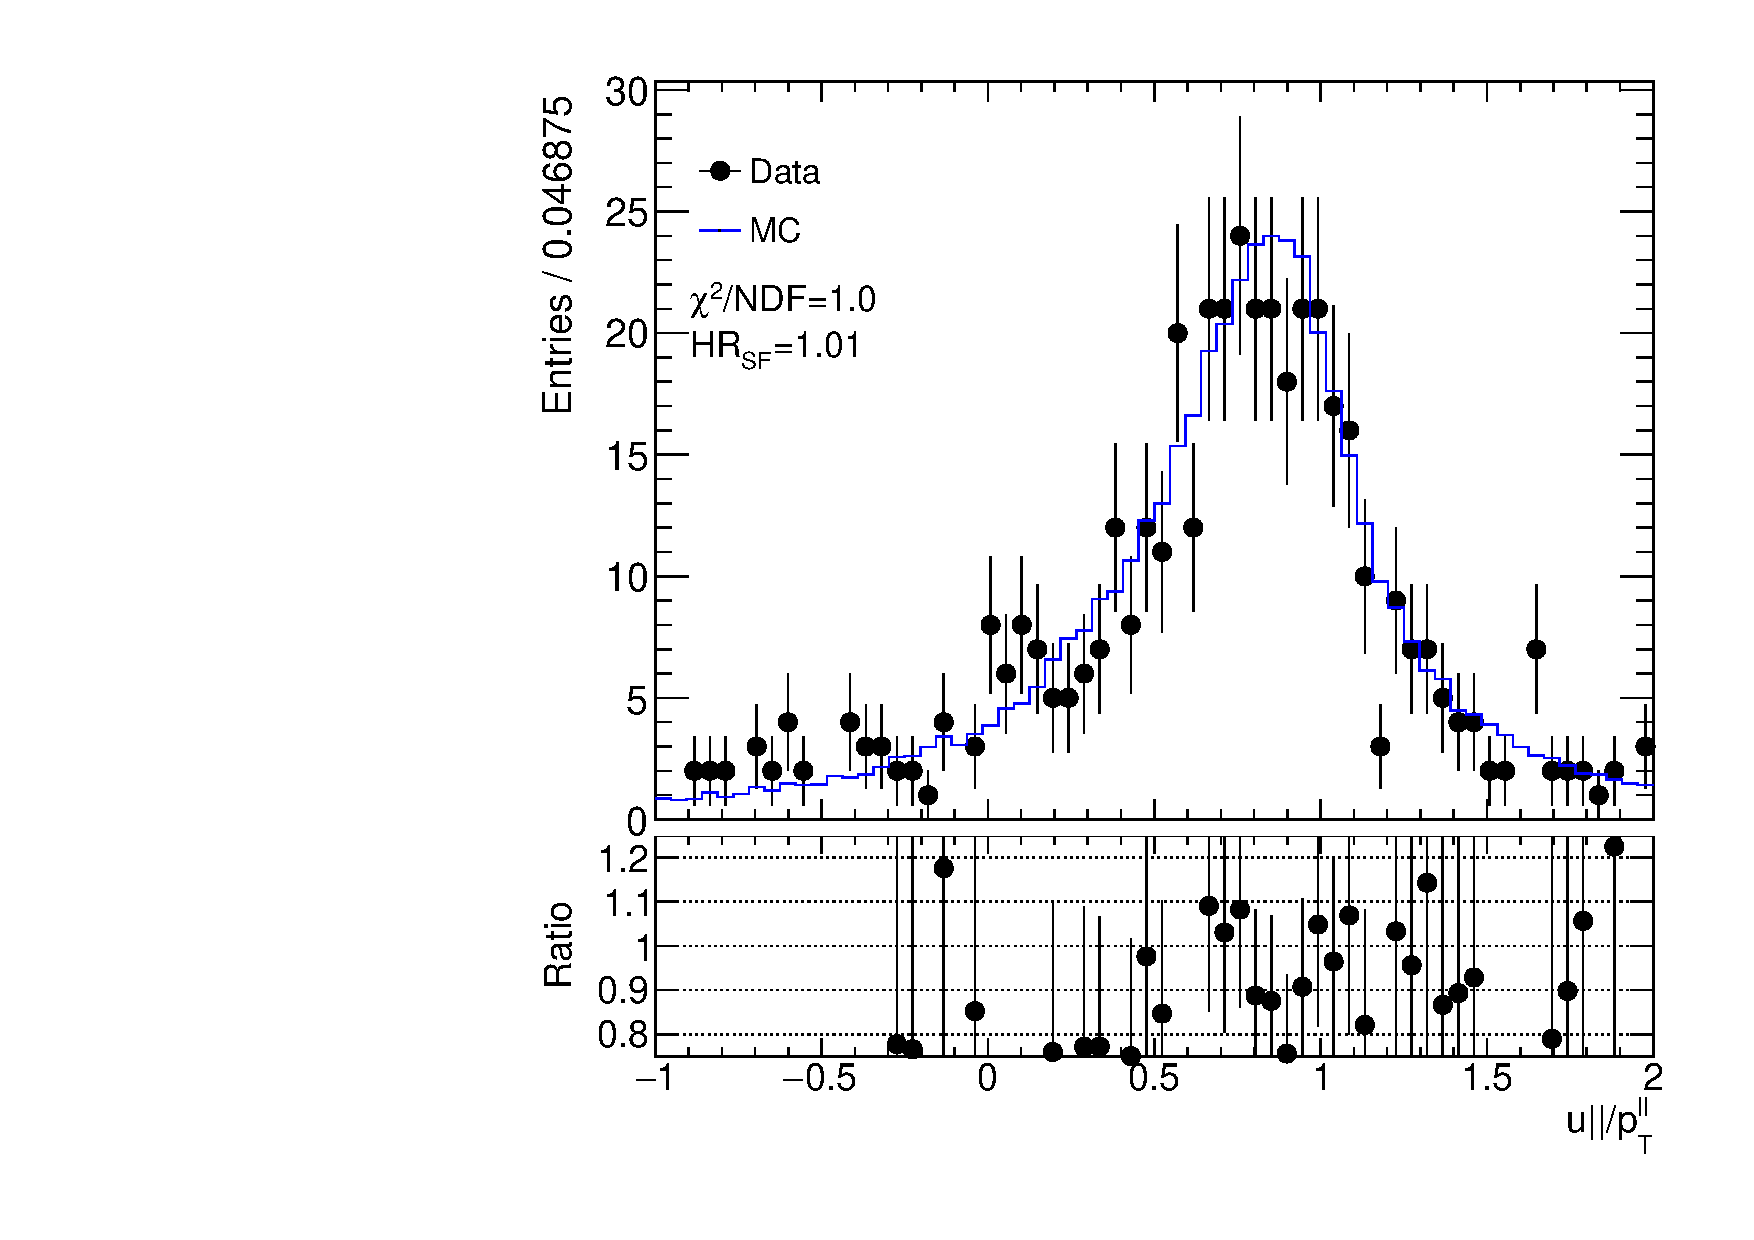
\includegraphics[width=\linewidth]{HadronRecoil/UParEScale13.pdf} b)}
\endminipage\hfill
\minipage{0.32\textwidth}%
   \center{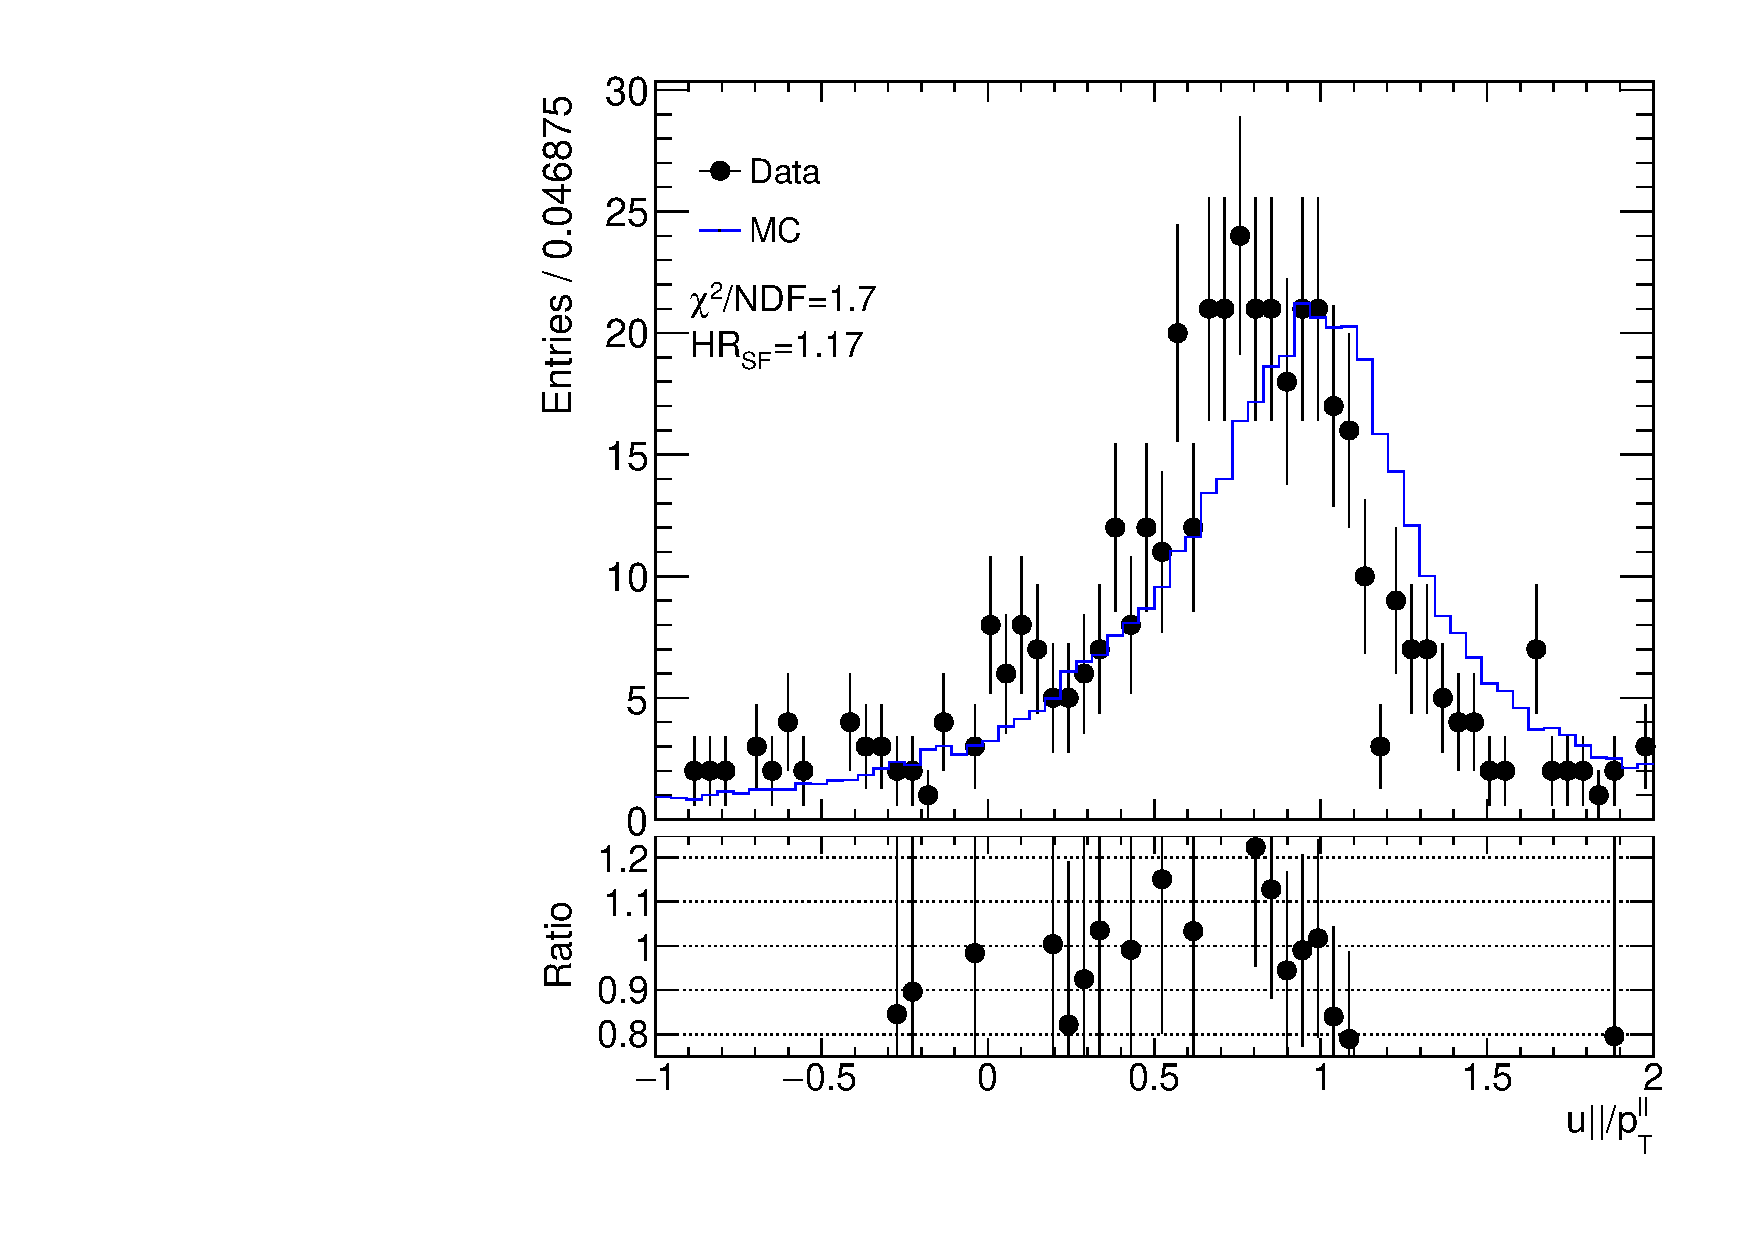
\includegraphics[width=\linewidth]{HadronRecoil/UParEScale21.pdf} c)}
\endminipage
\caption{}
\label{fig:MuSF}
\end{figure}
As it was mentioned before, it is possible to use both Z and W boson sample for hadron recoil bias determination. Correction factor $SF_{HR,bias}$ is applied as:
\begin{equation}
\upar^{MC,cor}=\upar^{MC} \cdot SF_{HR,bias},
\end{equation}

\begin{figure}[!tbp]
\begin{minipage}[h]{0.49\linewidth}
\center{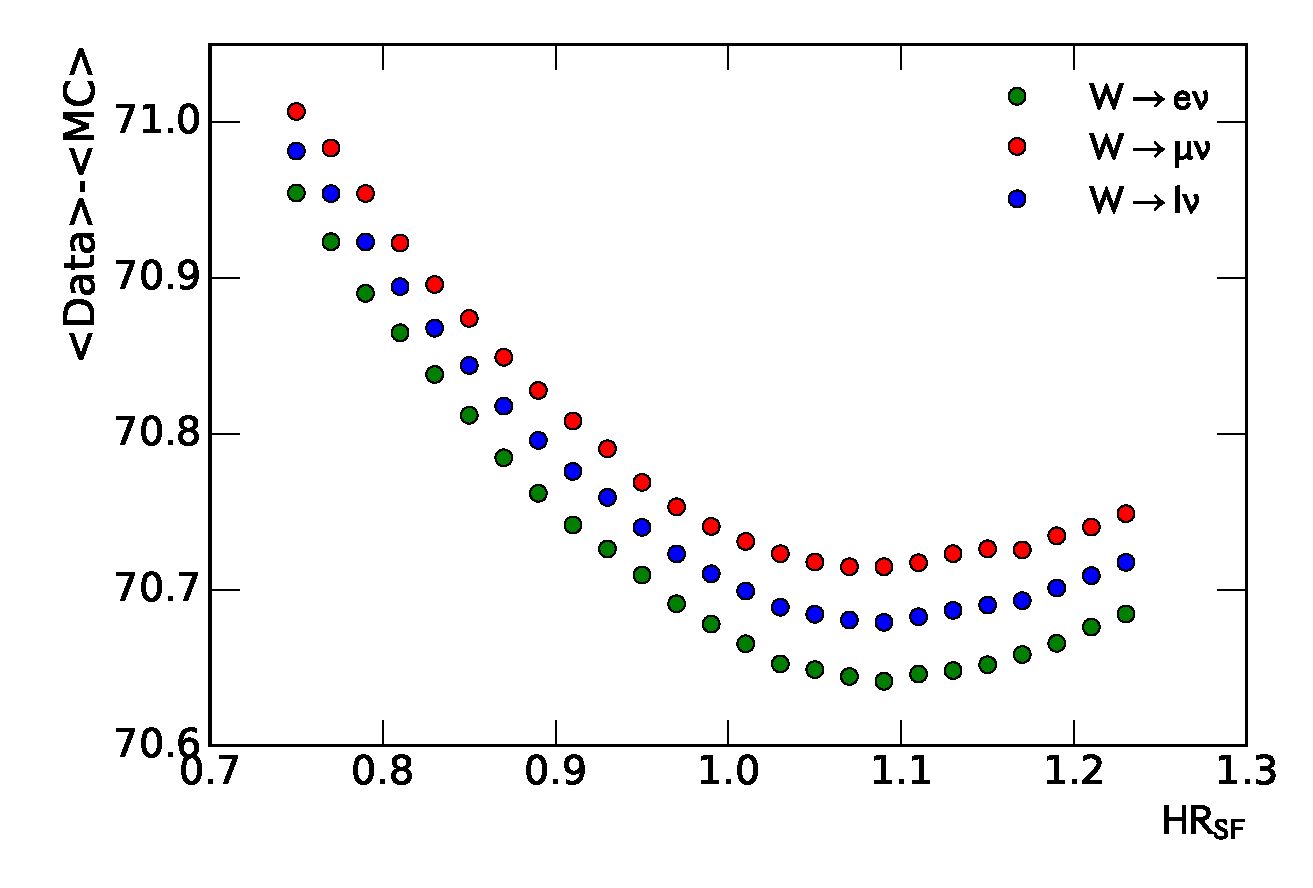
\includegraphics[width=1.\linewidth]{HadronRecoil/MeanAll.pdf} \\ a)}
\end{minipage}
\hfill
\begin{minipage}[h]{0.49\linewidth}
\center{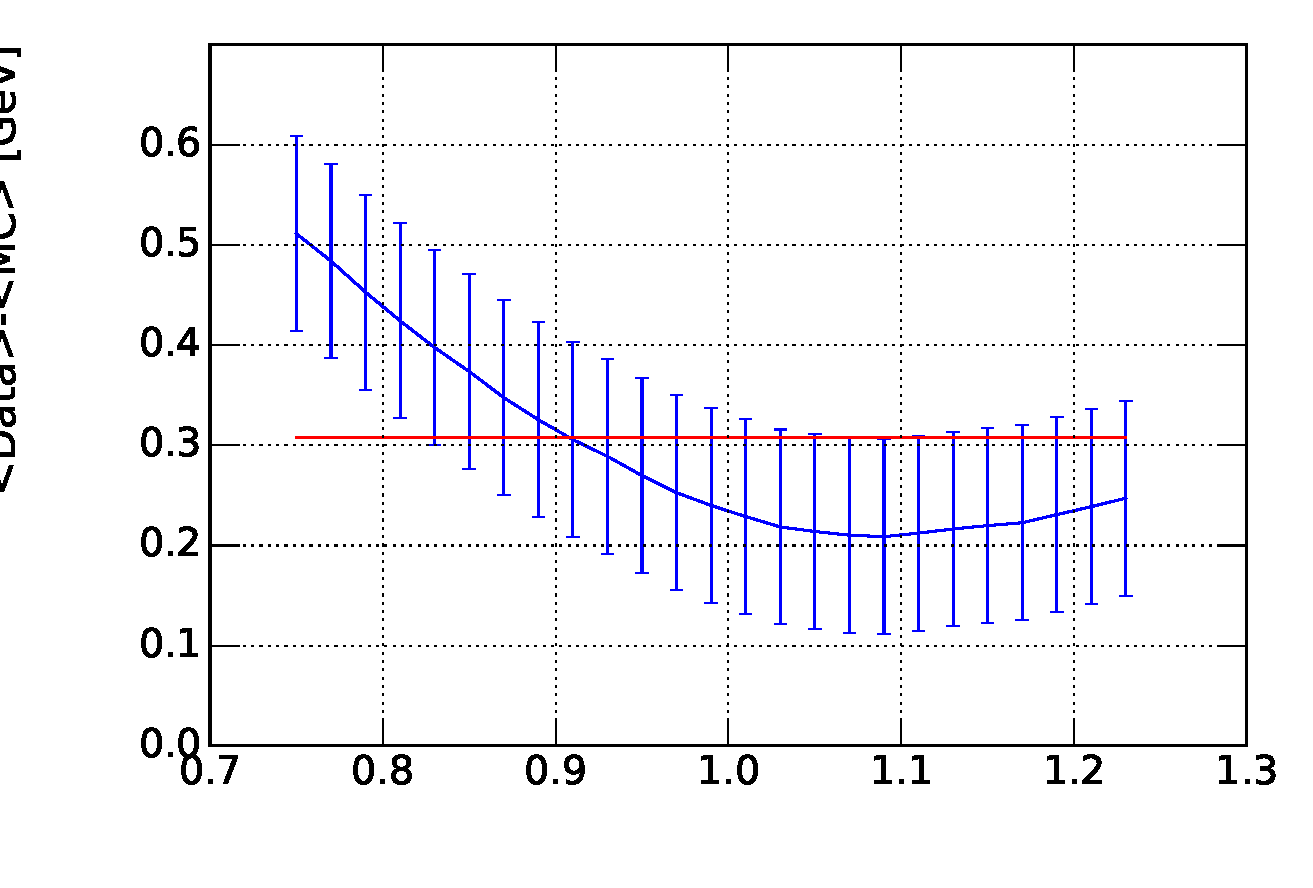
\includegraphics[width=1.\linewidth]{HadronRecoil/MeanCombined.pdf} \\ b)}
\end{minipage}
\caption{}
\vfill
\begin{minipage}[h]{0.49\linewidth}
\center{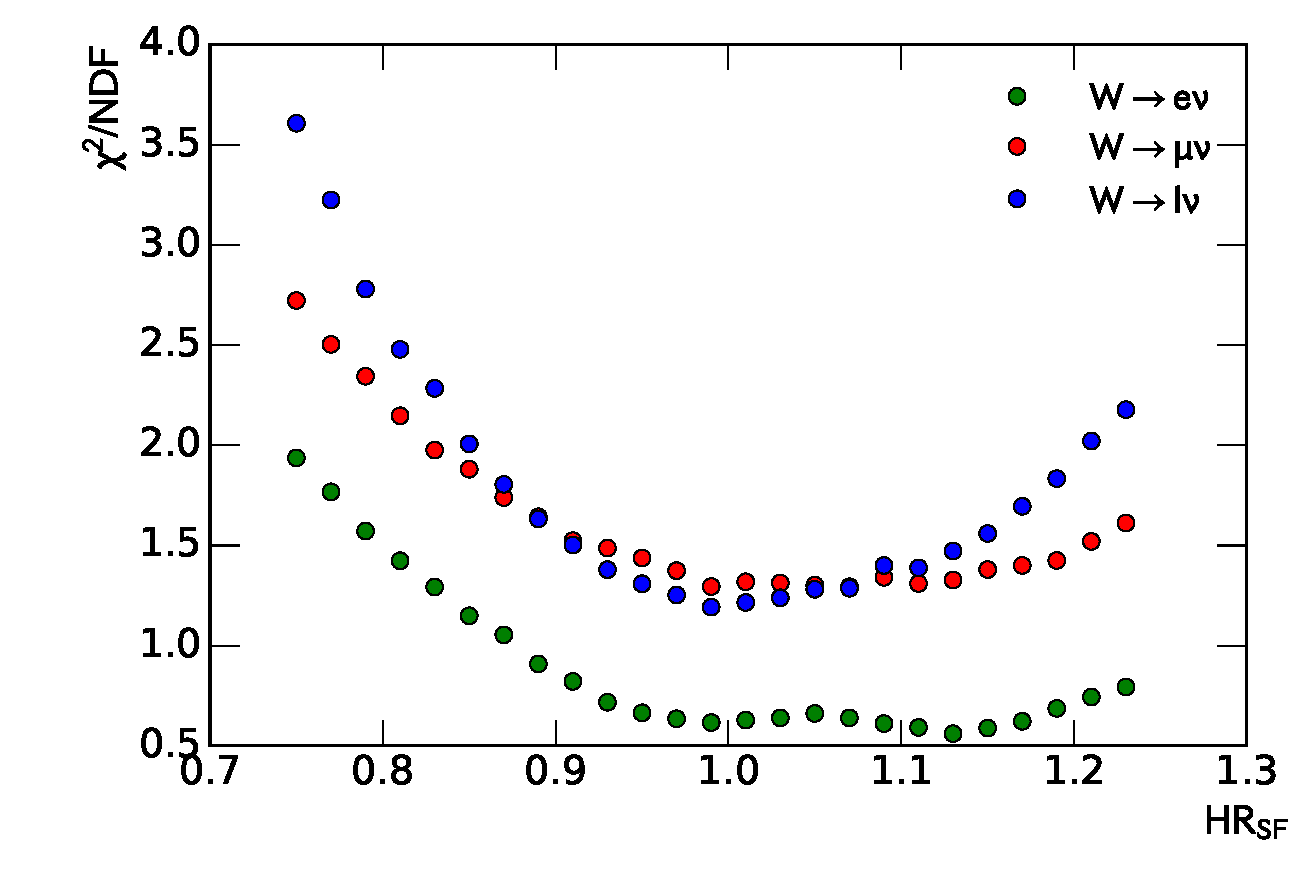
\includegraphics[width=1.\linewidth]{HadronRecoil/chi2AllChannelsMtw.pdf} \\ a)}
\end{minipage}
\hfill
\begin{minipage}[h]{0.49\linewidth}
\center{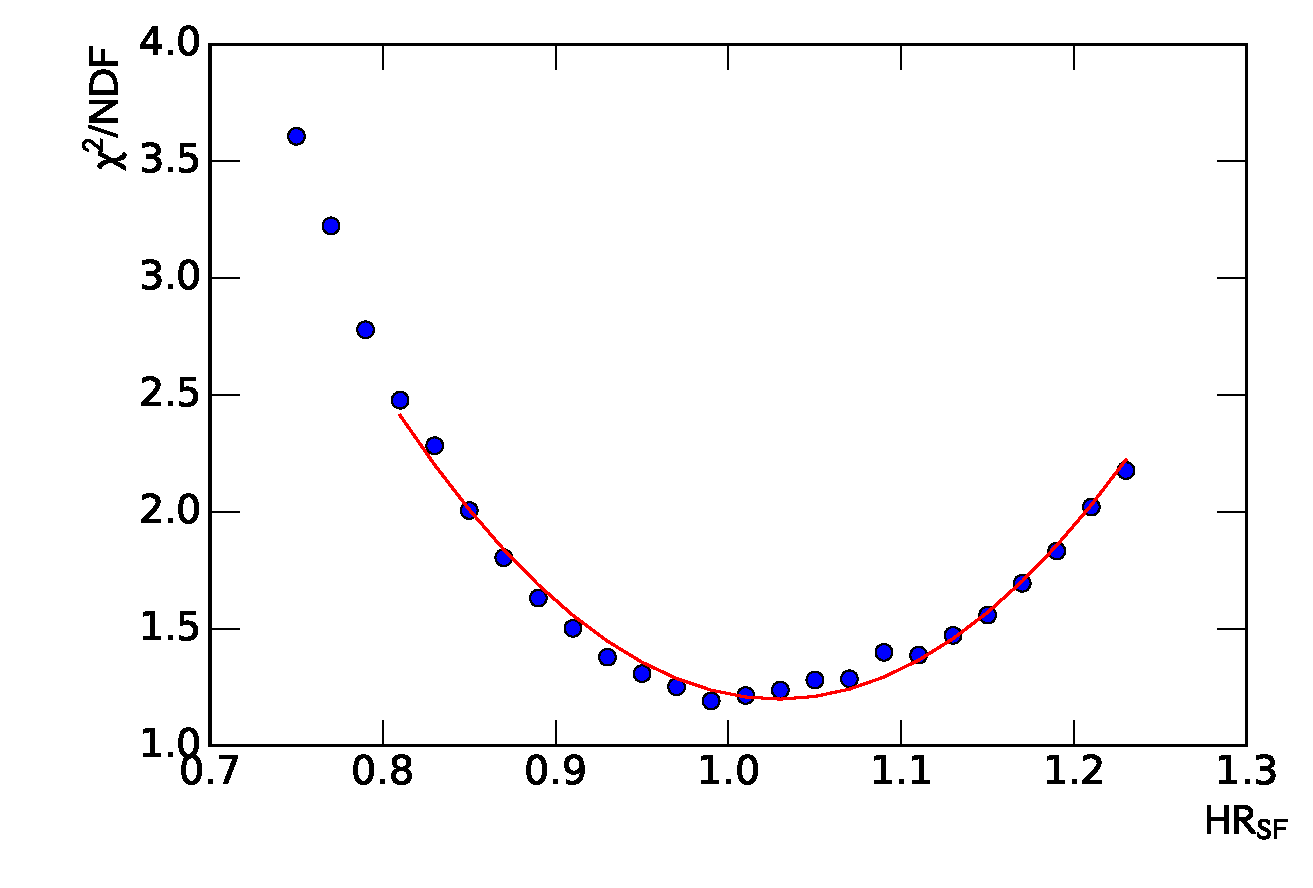
\includegraphics[width=1.\linewidth]{HadronRecoil/chi2TotalMtw.pdf} \\ b)}
\end{minipage}
\caption{}
\label{mtWChi2}
\end{figure}

\begin{figure}[!tbp]
\centering
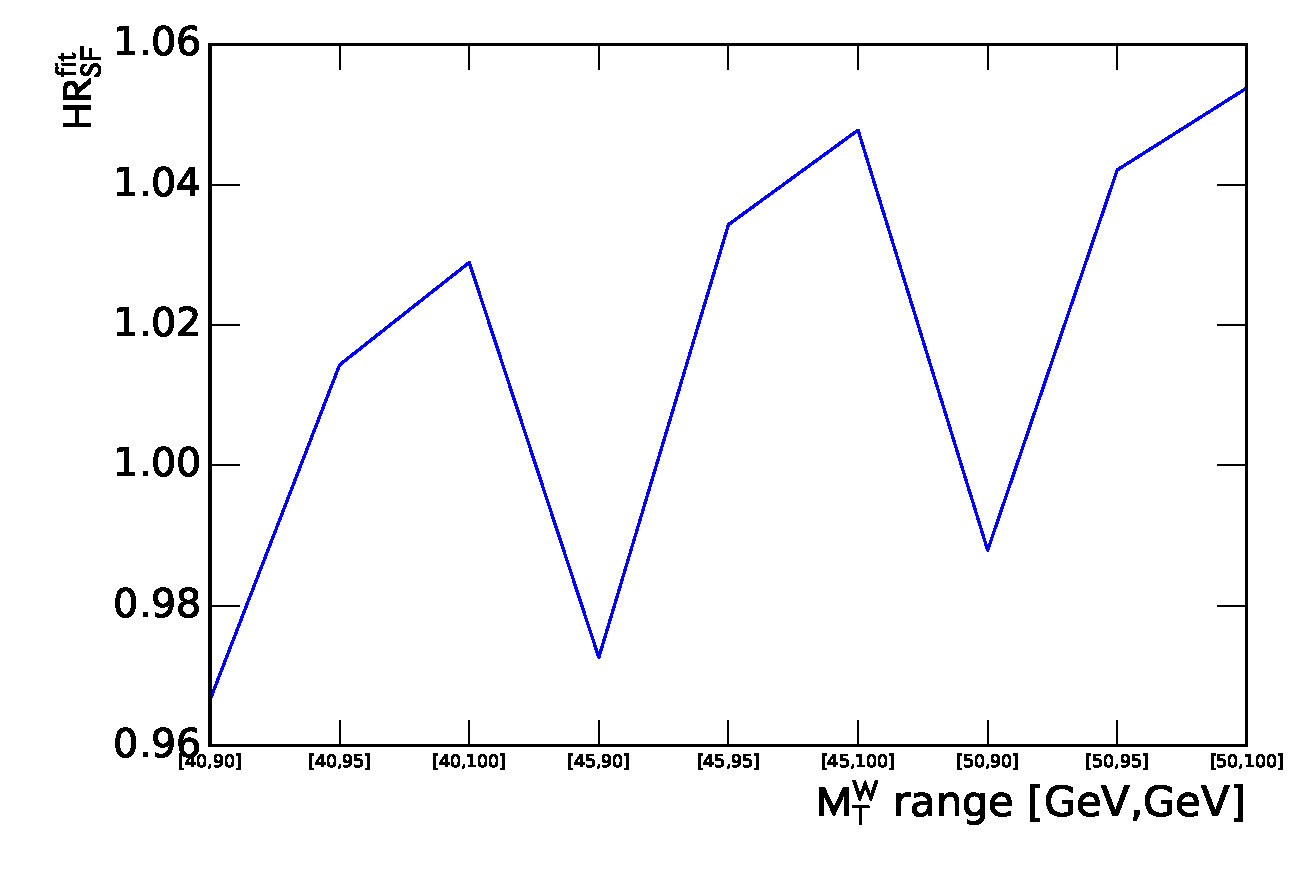
\includegraphics[width=0.7\textwidth]{HadronRecoil/RangeEffect.pdf}
\caption{}
\label{ScaleMtWRange}
\end{figure}

\begin{figure}[!tbp]
\begin{minipage}[h]{0.49\linewidth}
\center{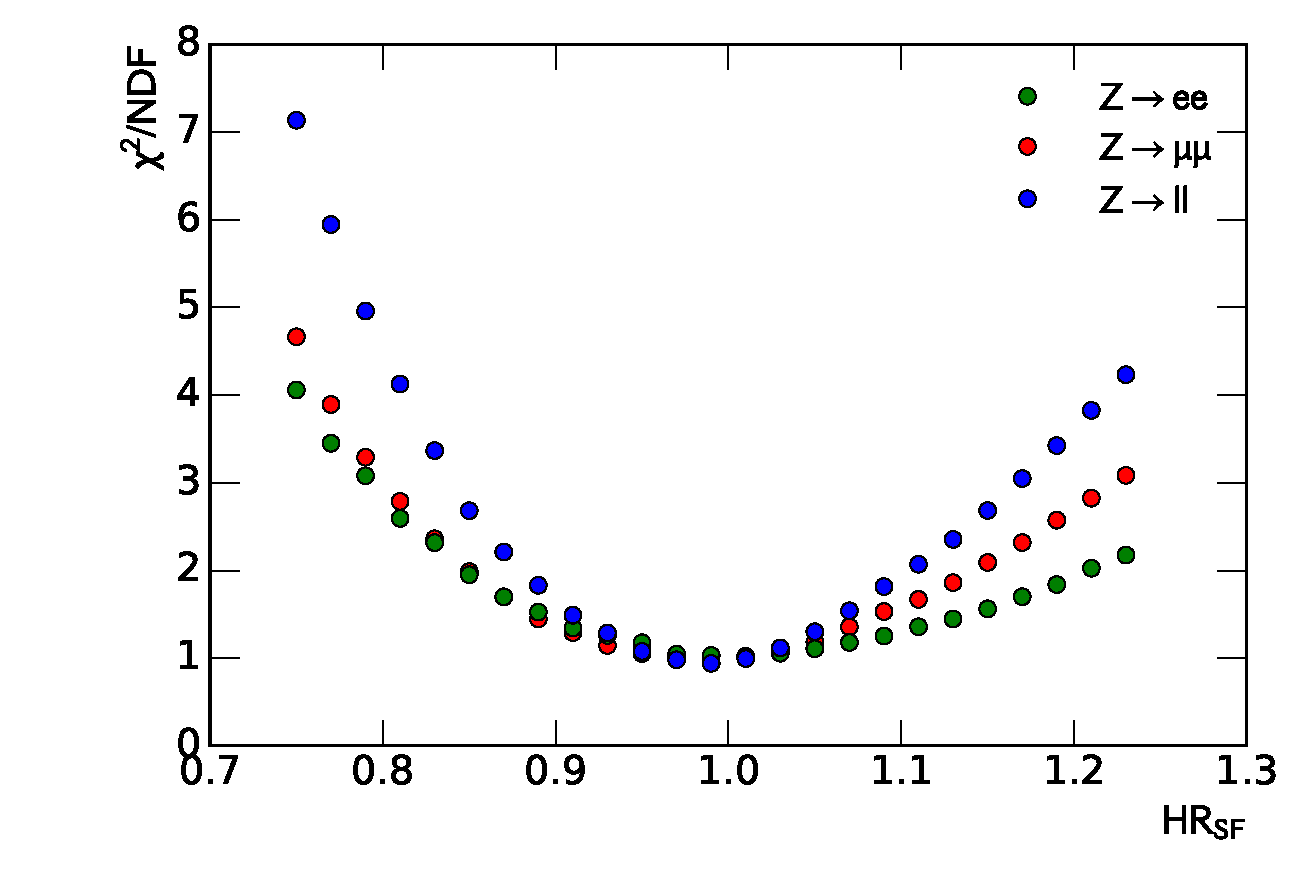
\includegraphics[width=1.\linewidth]{HadronRecoil/chi2Upar.pdf} \\ a)}
\end{minipage}
\hfill
\begin{minipage}[h]{0.49\linewidth}
\center{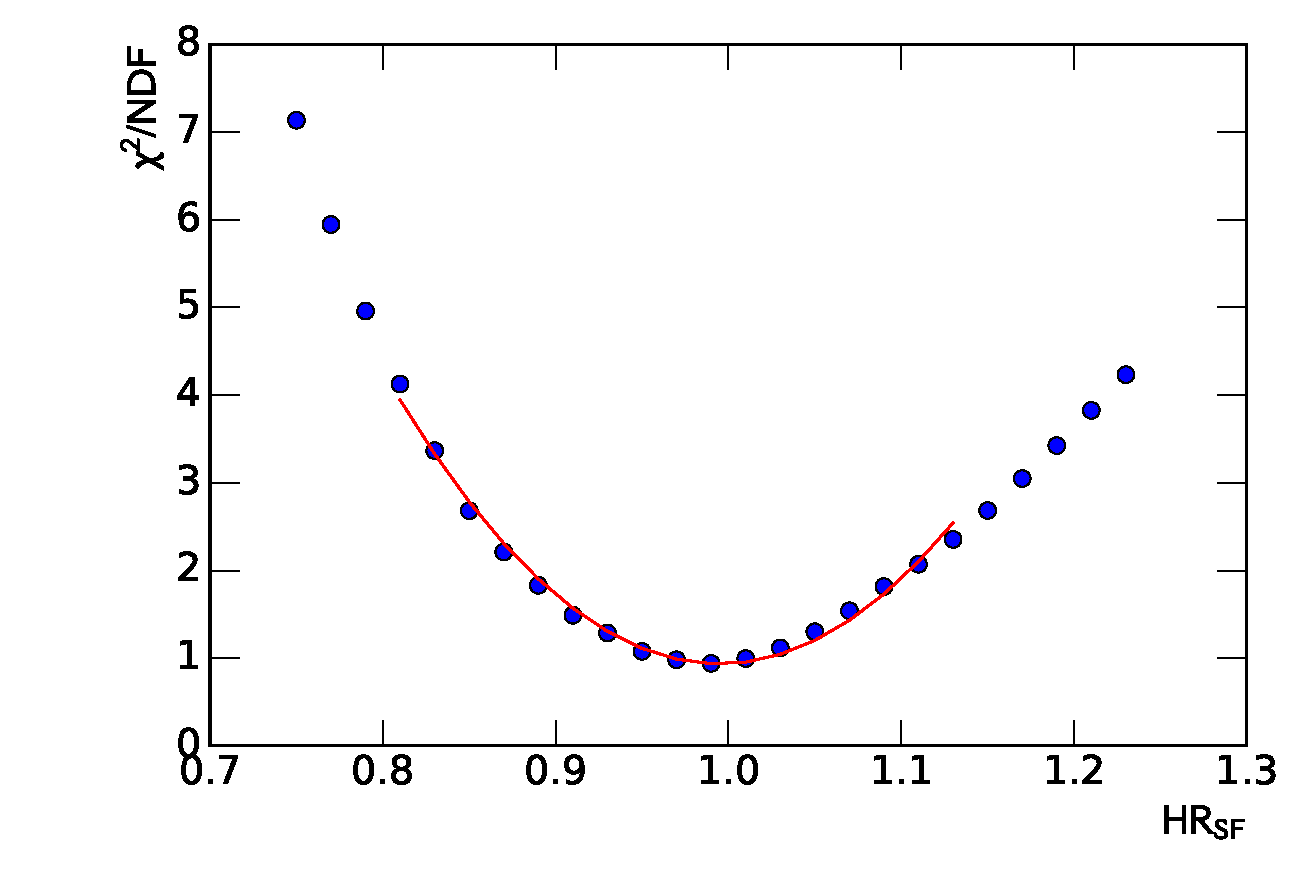
\includegraphics[width=1.\linewidth]{HadronRecoil/chi2UparTot.pdf} \\ b)}
\end{minipage}
\caption{Effect on a \cw for a different $d\sigma$ for a) \wenu b)\wmunu channel}
\label{uPAr}
\end{figure}
and can be obtained by scanning the impact of the scaling factor on the Data to MC agreement of the distributions that are dominated by the recoil scale uncertainties. Since W boson has no second source of \ptw measurments, determination of the hadron recoil bias should use the distributions, that  are not sensitive to a truth \ptw spectrum.  One of the optimal choises is a \mtw distribution. Transverse mass distribution for a different scale choises is shown on a Fig. \ref{HadronRecoilScaleMtW}. Multijet background is not included, because it shape and number of events is depending on a hadron recoil scale and thus can introduce additional systematics.

The first way to determine correction factor is using a difference in the mean of transverse mass in data and MC. Statistical error of this determination is an error of the mean in the data. The precision of this method is low, is it is mainly used as a cross-check. 

Second way is calculating \chiD for each correction factor. The ideal correction factor is determined by fitting \chiD distribution by the function:
\begin{equation}
\chi^2 = \frac{(x-sf_{best})^2}{\sigma_{sf}^2}+\chi^2_0,
\end{equation}
where $sf_{best}$ is the best scale factor and $\sigma_{sf}$ is a statistical error of this parameter. Distribution of \chiD and a fit in combined W channel is shown on a Fig. \ref{mtWChi2}.

Because of the possible mismodelling of the tail \mtw distribution it is not included in a \chiD calculation, leaving a free choice of the parameter of the cutoff.  It is also possible to exclude regions with high multijet background contamination by applying a tighter cut on a \mtw. 
This fit range is introducing one source of systematic error. Effect of the range on value determination is shown on a Fig. \ref{ScaleMtWRange}.
 
Similarly to a W channel, scale correction in a Z sample can be determined from distribution $\frac{\upar}{p_T^{ll}}$, shown on a Fig. \ref{uPAr}. 
Since there is no choise of the range and dependency on $P_T^{bos}$ modeling, there is just one source of uncertainty.
  
Results on a hadron scale factros and it's errors are shown in a Table \ref{tab:SFHadronRecoil}. The results are consistent within 1 sigma. 

\begin{figure}[!tbp]
\begin{minipage}[h]{0.49\linewidth}
\center{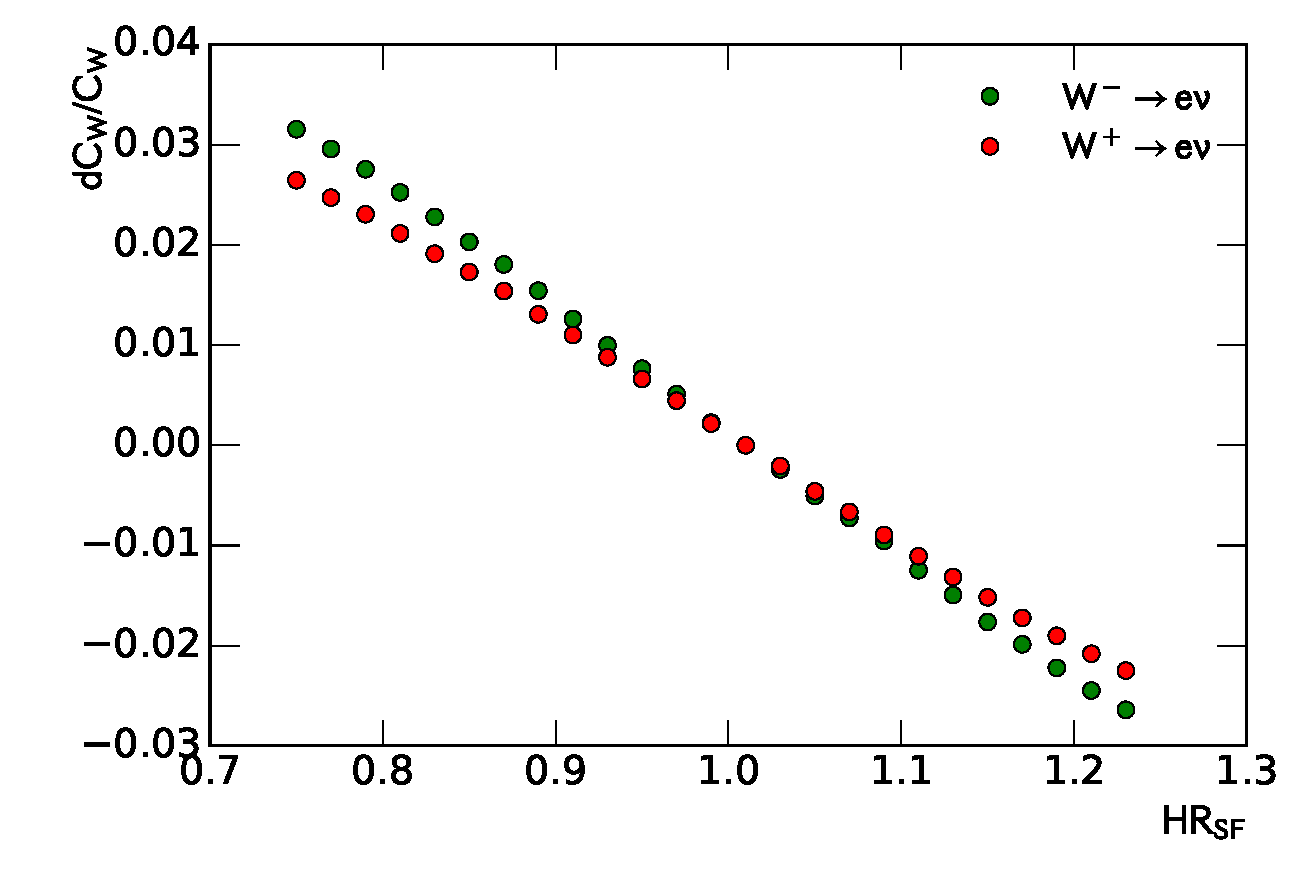
\includegraphics[width=1.\linewidth]{HadronRecoil/CWElectron.pdf} \\ a)}
\end{minipage}
\hfill
\begin{minipage}[h]{0.49\linewidth}
\center{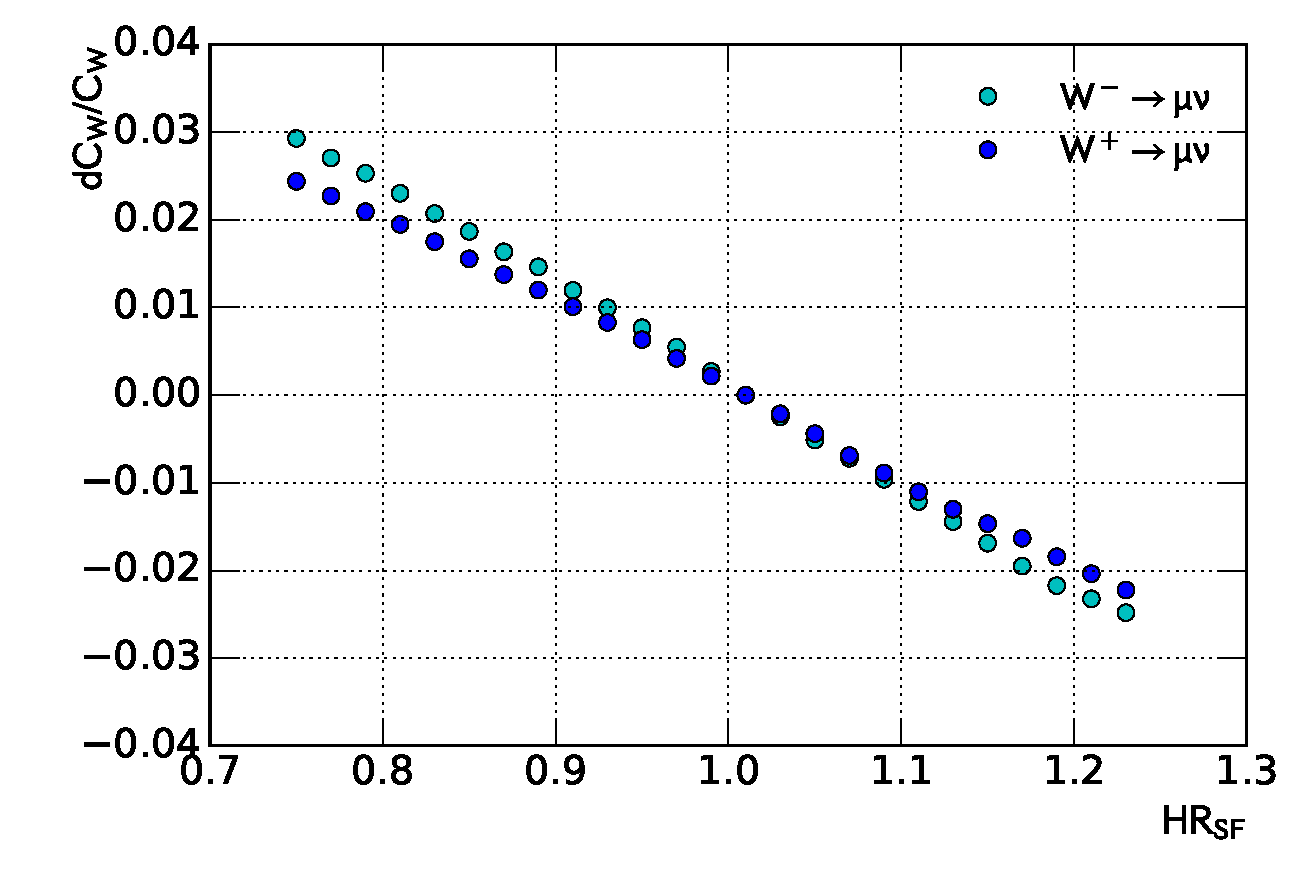
\includegraphics[width=1.\linewidth]{HadronRecoil/CWMuon.pdf} \\ b)}
\end{minipage}
\caption{Effect on a \cw for a different $d\sigma$ for a) \wenu b)\wmunu channel}
\label{ris:Cw}
\end{figure}

